\documentclass[
  a4paper,BCOR10mm,oneside,
  bibtotoc,idxtotoc,
  headsepline,footsepline,% also activate headinclude and footinclude
  fleqn,openbib
]{scrbook}
\usepackage[automark]{scrpage2}
\usepackage[ngerman,english]{babel}% default language as last entry
\usepackage[utf8]{inputenc}
\usepackage{amsmath} 
\usepackage{amsfonts}
\usepackage{amssymb}
\usepackage{graphicx}
\usepackage{lastpage}% to get last page use \pageref{LastPage}
\usepackage[refpage,intoc]{nomencl}% for nomenlature Abkuerzungsverzeichnis
\usepackage{listings}
\usepackage{color}
\usepackage{hyperref}
\usepackage{bm}
\definecolor{mygreen}{rgb}{0,0.6,0}
\definecolor{mygray}{rgb}{0.5,0.5,0.5}
\definecolor{mymauve}{rgb}{0.58,0,0.82}

\lstset{ %
  backgroundcolor=\color{white},   % choose the background color; you must add \usepackage{color} or \usepackage{xcolor}
  basicstyle=\footnotesize,        % the size of the fonts that are used for the code
  breakatwhitespace=false,         % sets if automatic breaks should only happen at whitespace
  breaklines=true,                 % sets automatic line breaking
  captionpos=b,                    % sets the caption-position to bottom
  commentstyle=\color{mygreen},    % comment style
  deletekeywords={...},            % if you want to delete keywords from the given language
  escapeinside={\%*}{*)},          % if you want to add LaTeX within your code
  extendedchars=true,              % lets you use non-ASCII characters; for 8-bits encodings only, does not work with UTF-8
  frame=single,	                   % adds a frame around the code
  keepspaces=true,                 % keeps spaces in text, useful for keeping indentation of code (possibly needs columns=flexible)
  keywordstyle=\color{blue},       % keyword style
  language=Octave,                 % the language of the code
  otherkeywords={*,...},           % if you want to add more keywords to the set
  numbers=left,                    % where to put the line-numbers; possible values are (none, left, right)
  numbersep=5pt,                   % how far the line-numbers are from the code
  numberstyle=\tiny\color{mygray}, % the style that is used for the line-numbers
  rulecolor=\color{black},         % if not set, the frame-color may be changed on line-breaks within not-black text (e.g. comments (green here))
  showspaces=false,                % show spaces everywhere adding particular underscores; it overrides 'showstringspaces'
  showstringspaces=false,          % underline spaces within strings only
  showtabs=false,                  % show tabs within strings adding particular underscores
  stepnumber=2,                    % the step between two line-numbers. If it's 1, each line will be numbered
  stringstyle=\color{mymauve},     % string literal style
  tabsize=2,	                   % sets default tabsize to 2 spaces
  title=\lstname                   % show the filename of files included with \lstinputlisting; also try caption instead of title
\makenomenclature
}

% define header and footer
\pagestyle{scrheadings}
\clearscrheadfoot % clear header and footer
\automark[section]{chapter}% !!! Wouldn't do that at oneside documents!!!
\ihead[]{\leftmark}% header left part
\ohead[]{\rightmark}% header right part
\ifoot{Name}% footer left part
\cfoot{Thema}% footer middle part
\makeatletter
% use different foot at front and main matter
\g@addto@macro{\mainmatter}{%
  \ofoot[{\usekomafont{pagenumber}Page \pagemark\ of \pageref{LastPage}}]
    {\usekomafont{pagenumber}Page \pagemark\ of 
      \pageref{LastPage}}% footer right part
}
\g@addto@macro{\frontmatter}{%
  \ofoot[\pagemark]{\pagemark}%
}
\makeatother


\begin{document}
\frontmatter% title pages are not numbered but counted!
\begin{titlepage}
  \raggedright% Use a different title style
  \null% page started
  \thispagestyle{empty}
  \selectlanguage{english}
  \vspace{4\baselineskip}
  \begin{tabular}{|ll@{}}
    & \\[\baselineskip]
    & \large Midtherm Report\\
    & \large Jan Grzegorzewski \\[\baselineskip]
    & \huge\textbf{Reaction-diffusion dynamics} \\
    & \huge\textbf{with fractional Brownian motion}\\[\baselineskip]
    & \large Summer term: 2016\\[2\baselineskip]
  \end{tabular}
\end{titlepage}

\tableofcontents
\listoffigures
\listoftables

\mainmatter
\selectlanguage{ngerman}
\selectlanguage{english}
\printnomenclature
\clearpage

\newtheorem{mydef}{Definition}
\newcommand{\norm}[1]{\left\lVert#1\right\rVert}

\chapter{Introduction}
Anomalous diffusion can be observed in many different areas of nature, in particular related to heterogeneous media (Crowded biological media, porous materials, ...). The most popular phenomenon of anomalous diffusion is a power-law behaviour of the Mean-Square-Displacement ($MSD\propto t^{\alpha}$), which is violating the Einstein formula $MSD=2 d D t$ and thereby the central limit theorem. Various theoretical models try to encounter the power-law behaviour of the MSD showing different origins for anomalous diffusion. These models have the main phenomenon, thus the power-law behaviour of the mean square displacement, in common. But differ in some other observables, due to different origins of the anomalous power-law behaviour. By measuring theses different quantities one might reveal the origin of the anomalous behaviour in an experiment.\newline
A basic model which accounts this phenomenon so far is Fractional Brownian Motion. This thesis is going to focus on Fractional Brownian Motion especially in respect to Reaction and Diffusion Dynamics. (Normal Diffusion Limited Smoluchowski equation, chemical master equation, mass action law michaelis menden reaction ????? check it ) is failing miserably in describing Reaction and Diffusion Dynamics while anomalous motion is present.(explain ...because of fluctuations). The overall work aims not only to bring Reaction Diffusion and Fractional Brownian Motion together but also providing a Fractional Brownian Motion Integrator implemented into a \textbf{Rea}ction \textbf{D}iffusion \textbf{Dy}namics software (ReaDDy). ReaDDy being a particle-based \textbf{Rea}ction \textbf{D}iffusion \textbf{Dy}namics software is acting on a macromolecular level. It is coarse-graining molecules into spherical particles. Usually using Brownian or Lagevin motion as the integrator. A Fractional Brownian Motion Integrator may be an elegant way of adding an approximation due to a crowded environment. The phenomenon of anomalous motion can also be studied with conventional integrators by actually building a crowded environment (for example: by adding obstacles). Nevertheless, the Fractional Brownian Motion approach could save computational time since it is not necessary to simulated each particle  explicitly which builds up the crowded environment. Furthermore different studies show that heterogeneous environments have influences on particle segregation in the presents of reactions.\newline
Having an Introduction set, chapter 2 deals with the theoretical foundation for Fractional Brownian Motion. Subsequently, due to computational reasons these theoretical elaborations need to be transferred into discrete space and finally casted into an algorithm. In the following some properties of the algorithm are studied.
In Chapter 3 theoretical foundation for reactions are going to be set. The final chapter 4 will deal with the present state of the thesis and give an outlook on further challenges.  

\chapter{Theory}
\section{Brownian Motion}
Fractional Brownian motion is a generalized case of standard Brownian Motion. The following section  will explore in more detail Brownian motion and normal diffusion. Than the more generalized case will be considerer. \newline
Standard Brownian Motion is a very important and good studied stochastic process. It describes the erratic motion for mesoscopic particles, which  first have been documented by Jan Ingenhousz in 1785, in particular for coal dust on the surface of alcohol. Later on in 1827 Robert Brown observed the erratic motion of pollen grains.  Brownian Motion has an Gaussian propagator which has its origin in the Central Limit Theorem (CLT) for a sum of of independent random variables. Lets assume a set of $N$ independent variables $\{X_i\}$ with a finite variance $ \sigma_i^2=\langle X_{i}^2\rangle $ and the mean $\langle X_{i}\rangle = 0$. The definition of a another random variable $Y$ is given by:
 \begin{align}
  Y = \frac{1}{\sqrt{N}} \sum_{j=1}^N X_j \label{eq:CLT}
 \end{align}
This scenario in which a random variable is defined of the sum of another can be observed generically in nature. In the following the distribution of Y, $\rho(y)dy=P(y<Y<y+dy)$ in the limit of large N, is going to be calculated. 
The Generating function for a random variable $Y$ is: 
\begin{align}
 G_Y(k)=\langle e^{ikY}\rangle = \int e^{ikY} \rho(y)dy
\end{align}
\ref{eq:CLT} can be inserted into the generating function, which results in:
\begin{align*}
G_Y(k)=\langle e^{\frac{ik}{\sqrt{N}} \sum_{j=1}^N X_j}\rangle \\
G_Y(k)=\langle \prod_{j=i}^N e^{\frac{ik}{\sqrt{N}} X_j} \rangle 
\end{align*}
If all $X_j$ are independent, then:
\begin{align}
 G_Y(k)= \prod_{j=i}^N \langle e^{\frac{ik}{\sqrt{N}} X_j} \rangle =e^{\sum_{j=1}^N A_j (\frac{k}{\sqrt{N}})} \\ \nonumber \text{ with } A_j(\frac{k}{\sqrt{N}})= ln \langle e^{\frac{ik}{\sqrt{N}} X_j} \rangle 
\end{align}
For large N behaviour, we assume $\frac{k}{\sqrt{N}} << 1$ and expand
\begin{align}
 A_j(\frac{k}{\sqrt{N}}) = ln(1+ \langle X_j \rangle \frac{ik}{\sqrt{N}} - \langle X_{j}^2 \rangle \frac{k^2}{2N}+\mathcal{O}(N^{- \frac{3}{2}}))
\end{align}
 with a finite variance $ \sigma_i^2=\langle X_{i}^2\rangle $ and the mean $\langle X_{i}\rangle = 0$
\begin{align}
 A_j(\frac{k}{\sqrt{N}}) = -\sigma_j^2 \frac{k^2}{2N}+\mathcal{O}(N^{- \frac{3}{2}}))
\end{align}

Thus, the generating function for large N is:

\begin{align}
 G_Y(k)=e^{- \frac{\sigma^2 k^2}{2}} \\ \nonumber
 \text{ with } \sigma =  \frac{1}{N} \sum_{j=1}^N \sigma_j^2 
\end{align}
The distribution of Y can be calculated via the inverse Fourier Transform:
\begin{align}
 \rho(y) &=\frac{1}{2 \pi} \int_{-\infty}^{\infty} e^{- \frac{\sigma^2 k^2}{2}} e^{i k y} dk \\  
 &=\frac{1}{\sqrt{2 \pi} \sigma } e^{-\frac{y^2}{2 \sigma^2}}
\end{align}
The seemingly innocent assumption of independence for the random variables $\{X_i\}$ in the summation result in an Gaussian distribution. Microscopic processes, which result in independent random position changes of an particle and add up over time, thus have a Gaussian distribution function for the overall position change.The propagator for Brownian motion has a Gaussian distribution.
\begin{mydef}
Standard Brownian motion is an stochastic process $ \{ W_t \}_{t\geq0}: \Omega \rightarrow \mathbb{R}^n$ with $ W_t(\omega)$ being the position of a particle with $\omega \in \Omega$ at time $t \in T$ in the observation time $T =[0, \infty)$. It has a fixed $x \in \mathbb{R}^n$ as its origin. For $ 0 \leq t_1 \leq ... \leq t_k, k \in \mathbb{N}, t_i \in T $ we define measures $\nu_{t_{1}... t_{k}}: \mathcal{B}(\mathbb{R}^n)^K \rightarrow [0,1]$. $\mathcal{B}$ is a borel set. The transition propabilities are: 
\begin{align}
T_{t}(y|x) & := (2 \pi t)^{- \frac{n}{2}} e^{- \frac{||x-y||^2}{2 t}} \text{for } y \in \mathbb{R}^n, t>0 \\ \nonumber
T_{0}(y|x) & = \delta(x-y) 
\end{align}
\end{mydef}
In the following some properties of Brownian motion are discussed:\\
\begin{itemize}
 \item Due to the Kolomogorov's continuity theorem a continuous path $ t \mapsto W_t(\omega)$ almost surely exists. Therefore it is possible to go to a continuous function $[0,\infty) \rightarrow \mathbb{R}^n$ and define a probability density.
\begin{align*}
p_{t_1,...,t_k}(x_1,...,x_k)  =T_{t_k -t_{k-1}}(x_k|x_{k-1}) ... T_{t_2 - t_1}(x_2|x_1) T_{t_1}(x_1|x)  \\
\text{ with }  0\leq t_1 < t_2 < ...< t_k,k \in \mathbb{N}
\end{align*}
\item Brownian motion is a Gaussian process with mean $E^x[W_t]=x$, $W_o=x$ 
Since $ E^x[(W_{t_i}-W_{t_{i-1}})(W_{t_j}-W_{t_{j-1}})]=0 $  all its increments $\{W_{t_1},W_{t_2}-W_{t_1},...,W_{t_k}-W_{k-1}\}$ are independent.

\item Brownian motion has stationary increments since ${W_{t-h}-W_{h}}$ has the same distribution for all $h>0$.

\item Brownian scaling $\{\hat{W}_t := \frac{1}{c} W_{c^2 t} \}_{t\geq0}$ if $\{W_t\}_{t \geq 0}$  is also a Brownian motion. Therefore Brownian motion has self-similar and fractal paths.
\end{itemize}
For Brownian motion a linear relation between the MSD and the diffusion constant can be shown. The starting point is the diffusion equation for overdamped motion with a constant diffusion coefficient $D$. 
\begin{align}
 \frac{\partial}{\partial t} C(x,t) = - \frac{\partial }{\partial x} J (x,t) = D  \frac{\partial^2 }{\partial x^2} C(x,t)
\end{align}
Flux of particles  $J(x,t)=\frac{\partial }{\partial x} C(x,t)$ as a result of a linear response relation. 
Under this approximation diffusion only depends on the position and not on the velocity. Therefore it is again a long-time approximation for normal diffusion. The propagator of Brownian motion solves this equation. The Concentration $C(x,t)$ can be in interpreted as a probability distribution if properly normalised as $\int dx C(x,t)=1$. The Mean Square Displacement (MSD) can be calculated as:
\begin{align}
 \frac{d}{dt} \langle x^2(t)\rangle & =\frac{d}{dt} \int dx x^2 C(x,t)=\int dx x^2 \frac{\partial}{\partial t} C(x,t) \\
&= D \int_{-\infty}^{\infty}dx x^2 \frac{\partial^2 }{\partial x^2} C(x,t) = -2 D \int_{-\infty}^{\infty} dx x \frac{\partial }{\partial x} C(x,t) \\ &= 2 D \int_{-\infty}^{\infty} dx C(x,t) =2 D
\end{align}
In previous equations partial integration has been used and  $C(\pm \infty,t)=0$ has been assumed.By integration for the initial condition $x(0) = 0$  one gets the Einstein Formula: $\langle (x(t)-x(o))^2)\rangle= 2Dt$, which can easily be extended for 2 and 3 dimensions. It will not be calculated here explicitly, but one can show that also for Smoluchowski eq. which follows from langevin dynamics for a long time limit the initial velocities decorrelates and thus the MSD is also linear with time.

\section{Fractional Brownian Motion}
In this section the theoretical foundation for Fractional Brownian Motion will be set and related to standard Brownian Motion. \\
In the previous section the the Means Square Displacement (MSD) has been shown to be linear with time as a result of the central limit theorem. In normal liquids this behaviour can be be seen already at time scales higher than picosecends \cite{Hofling2013}. Nevertheless many experiments show that the MSDs has a power law behaviour ( $\delta r ^2 (t) \propto t^{\alpha}$ for  $0 < \alpha < 1$ ). Thus the central limit theorem does not hold, not even for long time scales. It can be shown that persistent correlations of the increments can be observed. In soft matter,like polymers, subdiffusive behaviour is typically present in an time window but finally the linear MSD takes over. In particular Fractional Brownian Motion examines the case that the central limit theorem is violated for all time scales.\\
In the following some statistical tools are defined. They are important as the increments of Fractional Brownian motion are no longer assumed to be independent. The single particle density $\rho(\bm{r},t)=\delta(\bm{r}-\bm{R}(t))$ describes the density of a particle which is localized at position $\bm{R}(t)$, Its correlation function $P(\bm{r}-\bm{r}',t-t')= V\langle\rho(\bm{r},t) \rho(\bm{r}',t')\rangle$ is also called Van Hove self-correlation function. $V$ refers to the volume. From now on we will consider an isotropic system $ r= |\bm{r}|$. As for Brownian motion with independent increments the correlated increments  $\Delta\bm{R}(t)$ of fractional Brownian motion are assumed to follow a Gaussian distribution with zero mean.Thus the correlation function of the single particle density results in:
\begin{align}
 P(r,t)=[2 \pi \delta r^{2}(t)/d]^{-\frac{d}{2}} e^{ \frac{-r^2 d}{2 \delta r^{2}(t) }}
\end{align}
The van hove correlation function can be transformed via the spatial Fourier transform into the wave-number representation, which is called the self-intermediate scattering function. Again for isotropic systems one can write $|\bm{k}|=k$.
\begin{align}
 F_{s}(k,t)&=\langle\rho(k,t) \rho(k',t')\rangle=\int d^{d}r e^{-i k r} P(r,t) \\
 &=\langle e^{-i k \Delta R(t)} \rangle
\end{align}
The intermediate scattering function for the single particle density turns out to be the characteristic or moment generating function of $\Delta R(t)$ by expanding it for small wave-numbers $k \rightarrow 0$ one can get the moments. An other important quantity is the dynamical structure factor, which is the time-frequency Fourier transform of the intermediate scattering function:
\begin{align}
 F_{s}(\bm{k},z)&=\langle\rho(\bm{k},z) \rho(\bm{k}',z')\rangle=\int_{0}^{\infty} d t e^{-i \bm{k} \bm{r}} P(r,t) \text{ for } k \rightarrow 0 , \operatorname{Im}(z) > 0 \\
 &= \frac{1}{-iz}-\frac{k^2}{2d}\int_{0}^{\infty} d t e^{izt} \delta r^2 (t) + \mathcal{O}(k^2)
\end{align}
Another important correlation function is the Velocity Autocorrelation Function (VACF):
\begin{align}
Z(t)= \frac{1}{d}\langle \bm{v}(t) \bm{v}(0) \rangle 
\end{align}
 freqency represnetation of VACF

 non gaussian paramter 
From the observation of The Mean Square Displacement  $\delta r^{2}(t)= < \Delta R(t)>=2dK_{\alpha}t^{\alpha}$ one can calculated the velocity auto correlation function in the frequency domain as follows:

\begin{align*}
 \tilde{Z}(z)&=\int_{0}^{\infty} d t e^{izt} Z(t) \\
 &=2 d \int_{0}^{\infty} d t e^{izt} \left[\frac{d^2}{dt^2}\delta r^2 (t) \right]
\end{align*}
\begin{align*}
  \stackrel{par. integ.}{=} 2d \left( \underbrace{\left [ e^{izt}\overbrace{ \frac{d^2}{dt^2} 2dK_{\alpha}t^{\alpha}}^{=A(t)} \right]_{0}^{\infty}}_{\stackrel{\alpha < 2} {=} 0}-\int_{0}^{\infty} d t e^{izt} \left[\frac{d}{dt}\delta r^2 (t)\right] \right) 
 \end{align*}
 \begin{align*}
 A(t)=\frac{d}{dt}\overbrace{ \left [\frac{2d K_{\alpha}t^{\alpha-1}}{\alpha} \right ]}^{B(t)}=\frac{2d K_{\alpha}t^{\alpha-2}}{\alpha+(\alpha-1)}
\end{align*}

\begin{align*}
 \tilde{Z}(z) & \stackrel{par. integ.}{=} - 2d \left( \underbrace{\left [ e^{izt}\overbrace{ \frac{d}{dt} 2dK_{\alpha}t^{\alpha}}^{=B(t)} \right]_{0}^{\infty}}_{\stackrel{\alpha < 1} {=} 0}-\int_{0}^{\infty} d t e^{izt} \delta r^2 (t) \right) \\
  & = \int_{0}^{\infty} d t e^{izt} \delta r^2 (t)  \stackrel{\operatorname{Im}(z)> 0} {=}  K_{\alpha} \Gamma(1+\alpha)(i z)^{1-\alpha}
\end{align*}















Gebrochene Brownische Bewegung ist eine Verallgemeinerung der Brownischen Bewegung. Sie kann benutzt werden bei der Simulation von Anomaler Diffusion.\newline \newline
Theorie von Felix, bisschen von Christoph und die Motivation könnte sein, dass man zwar anomale Diffusion simuliert werden kann wenn man alle Teilchen berücksichtigt. Mit diesem Ansatz könnte man konkret den Einfluss von Gebrochen-rationale Brownische Bewegung auf Reaktionen test.zb.als Vergleich zu normaler Brownian motion und Brownian Motion an sich ist auch schon eine Vereinfachung, welche eine zufällige Gaußzahl annimmt. Das heißt sämtliche Stöße des Teilchens mit anderen Teilchen innerhalb eines Zeitinvervalls werden schon zu diesem Wert verallgemeinert. Als Unterschied zu tatsächlichen Simulation von allen Stößen (MD-Simulation).
Die Motivation ist einen performanten Integrator für gebrochen-rationale Brownische Bewegung zu entwickeln. Die Anomale Diffusion, welche besonders in biologischen Systemen zu beobachten ist, wird durch Interaktion der Teilchen mit ihrer Umgebung verursacht. Für den im Verlauf verwendeten Integrator muss davon ausgegangen werden, dass keine weiteren Interaktion (Potentiale) auftreten. Da zur Erstellung der Trajektorie ihre sämtlichen Inkremente im voraus durch gewöhnliche Brownische Bewegung erstellt werden müssen. Der Vorteil von der Methode ist ihre Performance.  
Der hier verwendete Algorithmus leitet sich vom Davies-Haste Algorithmus \cite{Craigmile2003} ab.
Dabei werden anfänglich alle Inkremente (Geschwindigkeiten) für gewöhnliches Braunische Bewegung erzeugt $\eta_{Br}(t)= v(t)$. Für die Entfernung eines Teilchens zu seinem Ursprung gilt  $\Delta R(t)_{Br} = R(t)- R(0)= \int^t_{0}dt' v(t')$. Es ergibt sich für die Mittlere Quadratische Quadratische Verschiebung: \newline $\delta r^{2}_{norm}(t)= < \Delta R(t)_{Br}>=2dDt$ mit $d =\text{Anzahl der Dimension}$, $D = \text{Diffusionskonstante}$ und $t=$ Zeit. Da gewöhnliche Brownische Bewegung einer Gaußverteilung folgt und ein Markowischer Prozess ist,lässt sich für den Propagator  folgende Gleichung aufstellen:
\begin{equation}
 P(r,t)=[2 \pi \delta r^{2}_{norm}(t)/d]^{-\frac{d}{2}} e^{ \frac{-r^2 d}{2 \delta r^{2}_{norm}(t) }}
\end{equation}
\section{Fractional Brownian Motion}
Als Ausgangspunkt wird weiterhin die Differentialgleichung $\partial \boldsymbol{R}(t) = \boldsymbol{\eta}(t)$ betrachtet. $\eta_i(t)$ ist in dem Fall aber nicht mehr delta korreliert in der Zeit, wie für einfache Brownische Bewegung. Für Gebrochen-rationale Brownische Bewegung wird eine dauerhaftes Korrelation angenommen, sodass die Mittlere Quadratische Verschiebung nicht mit der für Brownische Bewegung übereinstimmt, aber stattdessen eine exponentielle Abhängigkeit zur Zeit aufweist $\delta r^{2}_{fBr}(t)= < \Delta R(t)_{fBr}>=2dK_{\alpha}t^{\alpha}$. 
%Für die Mittlere Quadratische Verschiebung gilt allgemein $\delta r^{2}_{fBr}(t) = \int^t_{0}dt' v(t')$ ...
Die Geschwindigkeitsautokorrelationsfunktion für Gebrochen-rationale Brownische Bewegung kann wie folgt definiert werden:
\begin{equation}
Z(\omega)= K_{\alpha} \Gamma(1+\alpha)(i z)^{1-\alpha} \text{   für} 
\end{equation}
\begin{itemize}
 \item $K_{\alpha} =$ generalisierter Diffusions-Koeffizient 
 \item $\omega = $ Frequenz 
\end{itemize}
\cite{Hofling2013}
\subsection{Algorythm}
Für den im Verlauf verwendeten Integrator muss davon ausgegangen werden, dass keine weiteren Interaktion (Potentiale) auftreten. Da zur Erstellung der Trajektorie ihre sämtlichen Inkremente im voraus durch gewöhnliche Brownische Bewegung erstellt werden müssen. Der Vorteil von der Methode ist ihre Performance. Der hier verwendete Algorithmus leitet sich vom Davies-Haste Algorithmus \cite{Craigmile2003} ab. Die theoretischen Überlegung aus dem Theorieteil müssen für den Algorithmus in eine diskrete Form gebracht werden. \\Das Inkrement ist:
\begin{align}
\boldsymbol{\eta} (t) \longrightarrow \boldsymbol{\eta}_j  \text{  mit  } j=(0,1,2,...,n)  \text{  und  } n= \text{ Schrittanzahl}
\end{align}
Die dickgeschriebenen Inkremente $\boldsymbol{\eta}_j$ sind als Vektoren zu verstehen. Die Schreibweise wird im Verlauf so belassen.
Es ergibt sich für die Länge der Trajektorie:
\begin{align}
 \Delta \boldsymbol{R}_n =  \sum_{j=0}^n \boldsymbol{\eta}_j  \Delta t \label{eq:diskretdeltar}
\end{align}
 Der Algorithmus hat die Motivation die Inkremente $ \boldsymbol{\eta}_j$so zu generieren, dass sie die Eigenschaften der Gebrochen-rationale Brownische Bewegung wiederspiegeln und sie insbesondere dem potentiellen Abklingen der Mittleren Quadratischen Verschiebung folgen.
\begin{align}
< \Delta \boldsymbol{R}_{fbr}>=2dK_{\alpha}t^{\alpha}
\end{align}
Der verwendete Algorithmus geht wie folgt:
 
\begin{enumerate}
 \item Es werden $2 n$ unabhängige Normalverteilte, mit dem Mittelwert $<\boldsymbol{n_j}>=0$ und der Standartabweichung $\delta \boldsymbol{n_j} = \sqrt{\Delta t}$, Zufallszahlen erstellt: 
 \begin{align}
  \boldsymbol{\eta_j}=(\boldsymbol{\eta_0},\boldsymbol{\eta_1},\boldsymbol{\eta_2},...,\boldsymbol{\eta_{2n}})= \boldsymbol{\mathcal{N}}(0,\sqrt{\Delta t}) \text{  mit  } j=(0,1,2,...,2n)
 \end{align}
Im Verlauf des Algorithmus wird die Motivation für die doppelte Anzahl an Zufallszahlen gegenüber der resultieren Trajektorienlänge für gebrochen-rationalen Brownische Bewegung erläutert.
 \item Die Inkremente werden dann mit Hilfe einer diskreten Fouriertransforamtion (numpy.fft) in den Frequenzraum transformiert.
 \begin{align}
  \boldsymbol{\eta_g}=\sum_{j=0}^{2n-1} \boldsymbol{\eta_j} e^{\frac{- i 2 \pi  j g }{2n}} \text{ mit } g = (0,1,2,...,2n) \\ 
  \end{align}
 Die entsprechende analytische Fouriertransformation ist:
 \begin{align}
  \boldsymbol{\eta}(\omega)=\int_0^{\infty}e^{- i 2 \pi \omega t}  \boldsymbol{\eta}(t) dt  \label{eq:diskret-freq1} \\
 \text{mit }\omega = g \Delta \omega \text{ , } \Delta \omega =  \frac{1}{2n \Delta t} \text{ und } t=j \Delta t \ \label{eq:diskret-freq}
 \end{align}
 
 \item Daraufhin wird die Auto-Korrelation Funktion \text{\cite{Hofling2013}} angewendet, wodurch die Inkremente jetzt einen gebrochen-rationalen Brownischen Charakter bekommen: 
 \begin{align}
  \boldsymbol{\eta_{fbr_g}}&=\boldsymbol{\eta_g} \sqrt{2 Re(Z_g)} \label{eq:corelastion} \\
  Z(\omega)&= K_{\alpha} \Gamma(1+\alpha)( - i \omega)^{1-\alpha}
  \end{align}
  $Z(\omega)$ wurde durch die analytische Fouriertransformation $Z(\omega)=\int_0^{\infty}e^{i \omega t} Z(t) dt$ bestimmt. Da Numpy FFT eine andere Definition der Fouriertransformation  benutzt (siehe Formel \ref{eq:diskret-freq1}), \\ wird  $Z'(\omega)=\int_0^{\infty}e^{- i2 \pi \omega t} Z(t)dt= K_{\alpha} \Gamma(1+\alpha)(i \omega 2 \pi)^{1-\alpha}$ so umgeschrieben. Im Anschluss wird $Z(\omega) \longrightarrow Z_g$ (nach Formel \ref{eq:diskret-freq} ) in eine diskrete Form gebracht.
  \begin{align}
  \longrightarrow Z_g&= K_{\alpha} \Gamma(1+\alpha)(i 2 \pi g \Delta \omega)^{1-\alpha} =  K_{\alpha} \Gamma(1+\alpha)(i g \frac{ \pi}{n \Delta t})^{1-\alpha} 
 \end{align}
 \item Für gebrochen-rationale Brownischen Bewegung ist die Auto-Korrelations Funktion  an der Stelle 0: $Z_{g=0}=0$. Daraus folgt nach Formel \ref{eq:corelastion}, dass auch das Nullte Inkrement im Frequenzraum $\boldsymbol{\eta_{fbr_{g=o}}}= 0$ ist. Das Nullte Inkrement im Frequenzraum ist mit Formel \ref{eq:diskretdeltar} aber auch:
 \begin{align}
  \boldsymbol{\eta_{fbr_{g=o}}} = \sum_{j=0}^{2n-1} \boldsymbol{\eta_j} e^{0}=\frac{\Delta  \boldsymbol{R}}{\Delta t}
 \end{align}
$\Delta \boldsymbol{R} $ ist in dem Fall die zurückgelegt Entfernung nach $2n$ Zeitschritten.
Dadurch würde das Teilchen nach $2n$ Schritten wieder zurück an seinen Ursprung kehren. Stattdessen wird Das Nullte Inkrement im Frequenzraum folgendermaßen berechnet:
\begin{align}
\boldsymbol{\eta_{fbr_{g=o}}} = \mathcal{N}(0,\sqrt{2 K_{\alpha} (2n \Delta t)^\alpha})
\end{align}
 gerechnet. Dies wäre korrekt, wenn Gebrochen-rationale Brownische Bewegung ein Markowischer Prozess wäre. Da dies nicht der Fall ist, entsteht an dieser Stelle eine Approximation. Um sie genauer zu verstehen muss ich mich damit noch weiter beschäftigen. Um den Einfluss der Approximation zu verringern wurde in Schritt 1 die doppelte Menge an Inkrementen erstellt. Die Hoffnung ist, dass der Einfluss der Approximation  mit zunehmender Entfernung von $2 \Delta R_{fbr}$ immer geringer wird und bei $\Delta R_{fbr}$ bereits vernachlässigbar ist.
 %\item Laut dem Davies Harte Algorithmus wird außerdem das n-te Inkrement im Frequenzraum %umgeändert:
 %\begin{align}
 %\eta_{fbr_{g=n}} =\sqrt{Re(Z_g 2 n)} \mathcal{N}(0,1) 
 %\end{align}
 % Noch nicht verstanden warum!!
 \item In der Zeitdomäne ergeben sich die Inkremente durch die Rücktransformation als:
 \begin{align}
 \boldsymbol{\eta_{fbr_j}}= \frac{1}{2n} \sum_{g=0}^{2n-1} \boldsymbol{\eta_g} e^{\frac{2 \pi i j g }{2n}}
 \end{align}
Es wird nur die erste Hälfte der Inkremente, $\eta_{fbr_j}$ für $j=(0,1,..,n)$, weiter verwendet.
\end{enumerate}
Für die drei dimensionale Gebrochen-rationale Brownische Bewegung kann für jede kartesische Komponente der soeben beschriebene Algorithmus verwendet werden, da davon ausgegangen wird, dass die Kartesischen Komponenten der Inkremente untereinander nicht korreliert sind. 
\subsubsection{Analyse of Algorythm}
Hier kommen die Plots  aus dem Analyse Skript rein.

\begin{figure}[h]
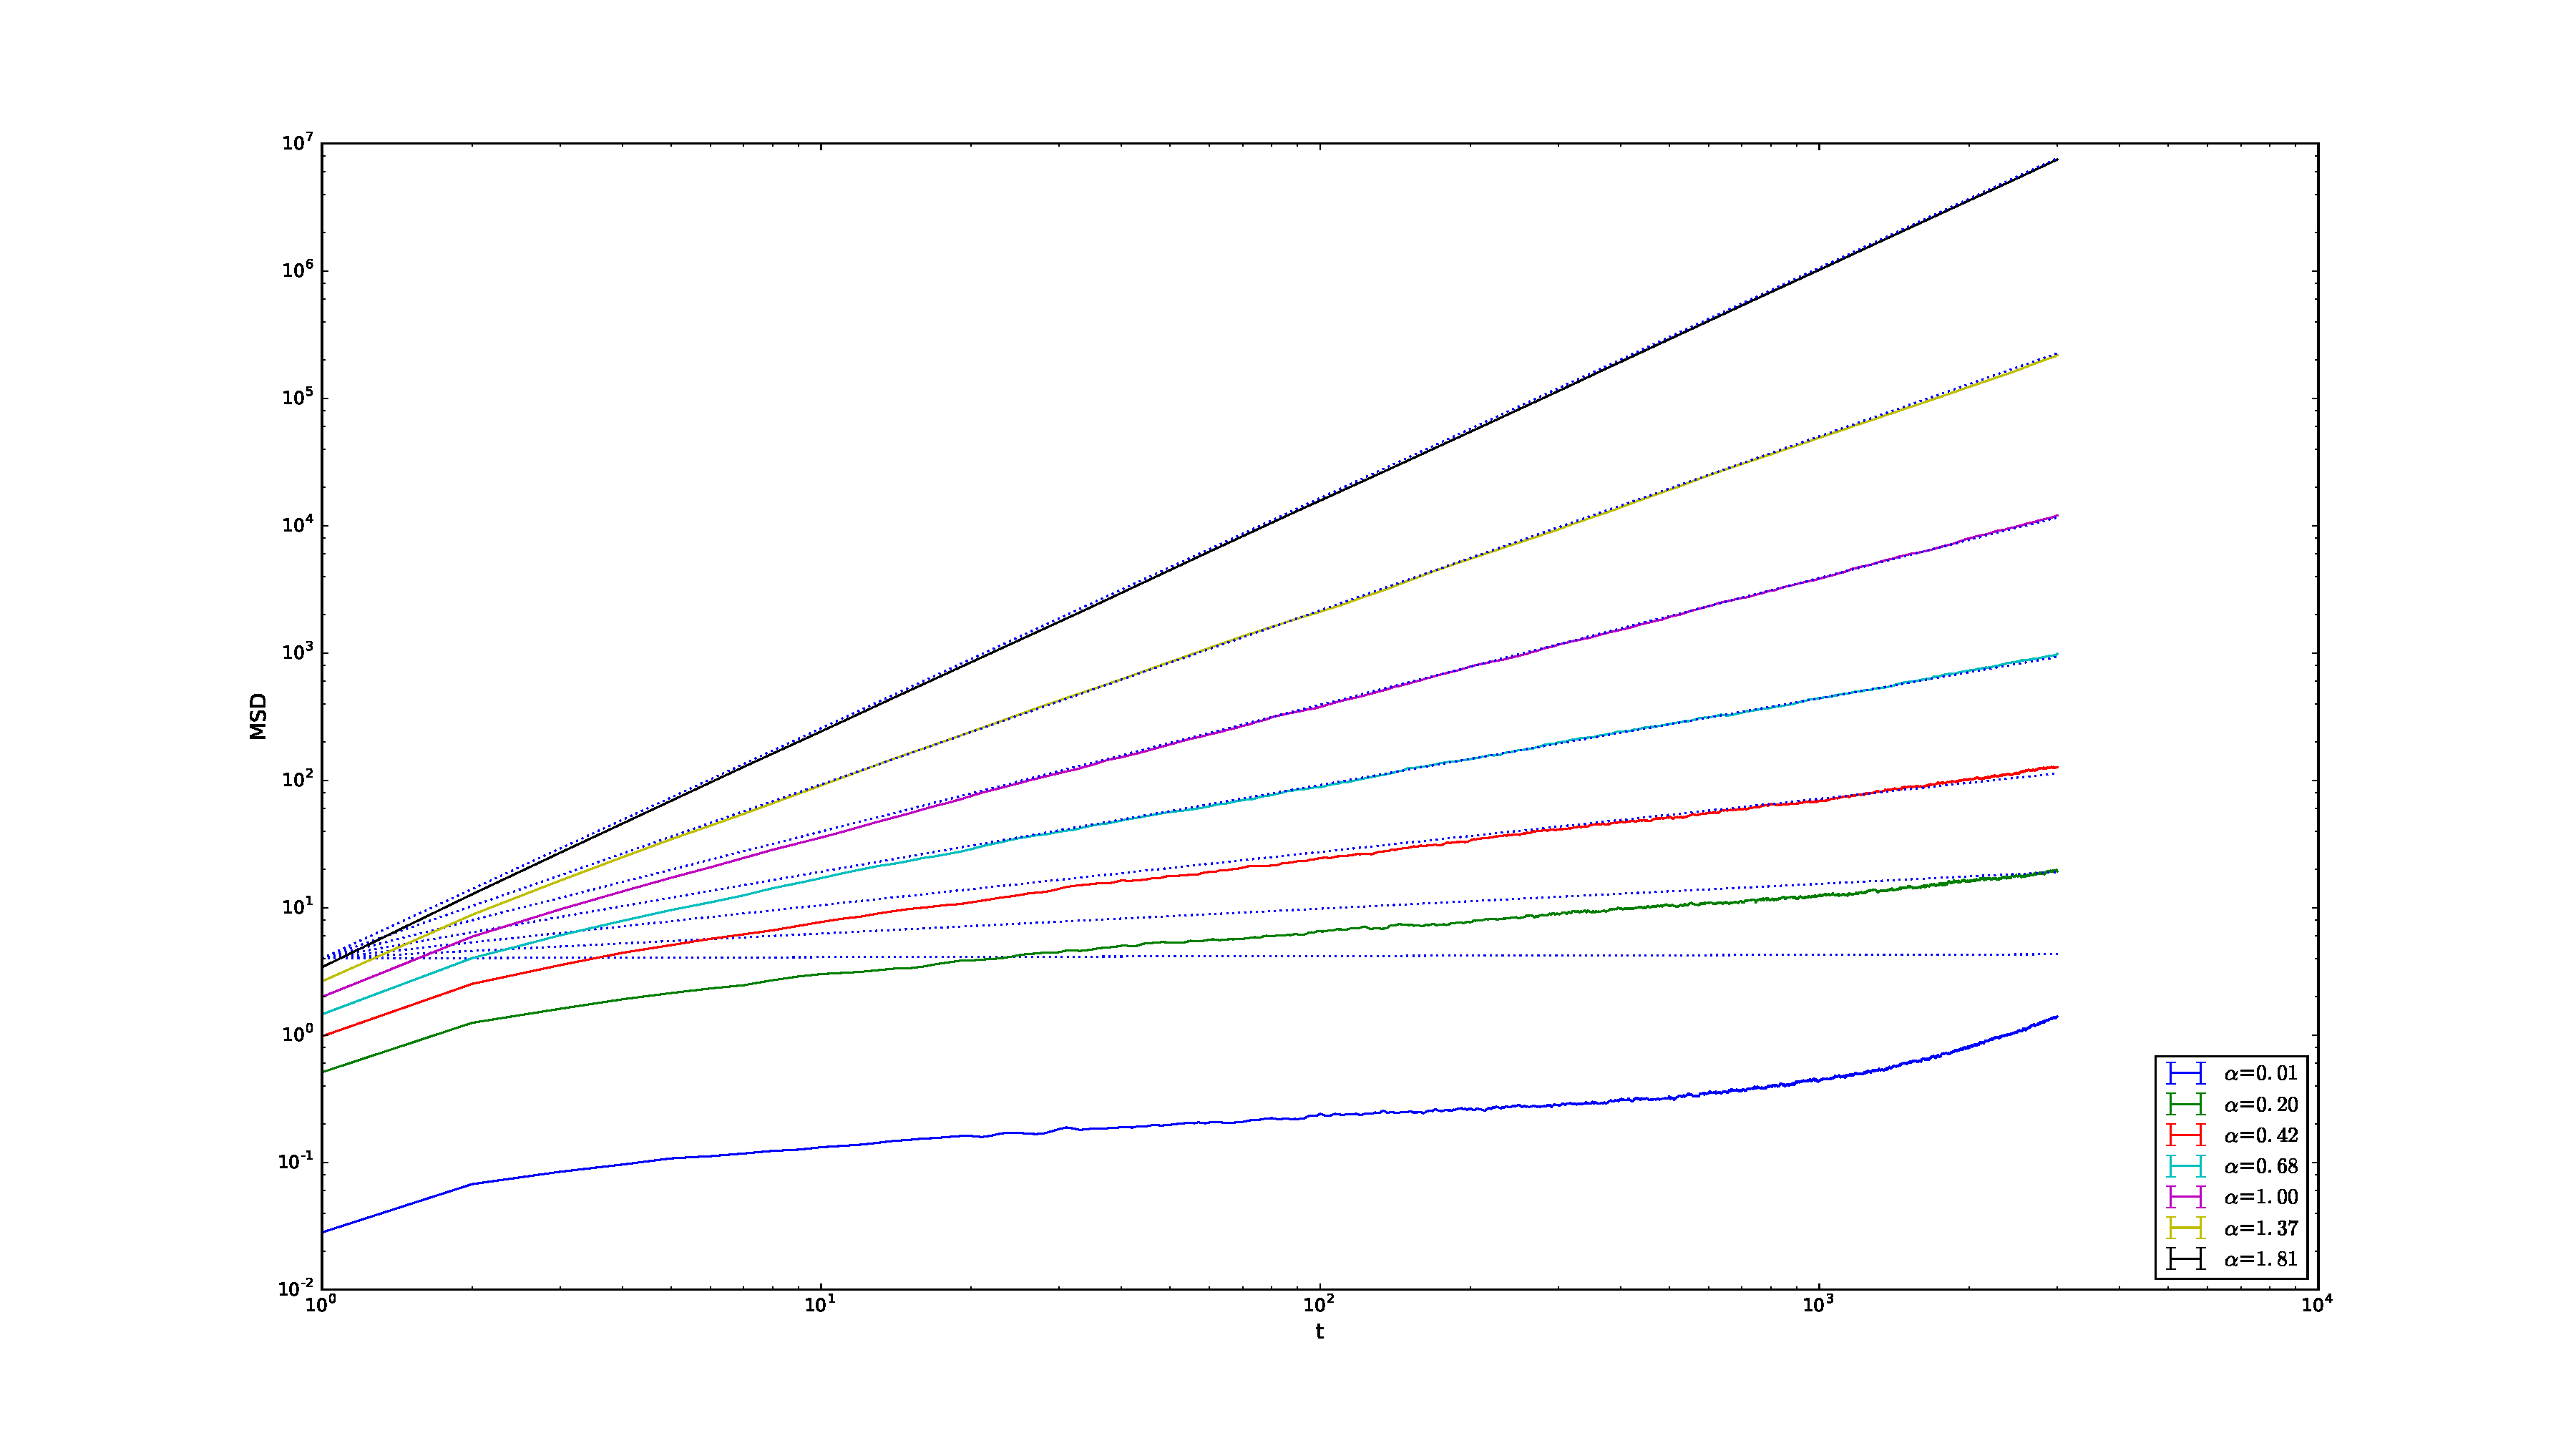
\includegraphics[width=\textwidth]{./msd_ensemble_alpha.pdf}
\caption{Mean Square Displacement of different $\alpha$}
% msd_ensemble_4000particles_log.pdf: 0x0 pixel, -2147483648dpi, 0.00x0.00 cm, bb=
 \centering
\end{figure}


\begin{figure}[h]
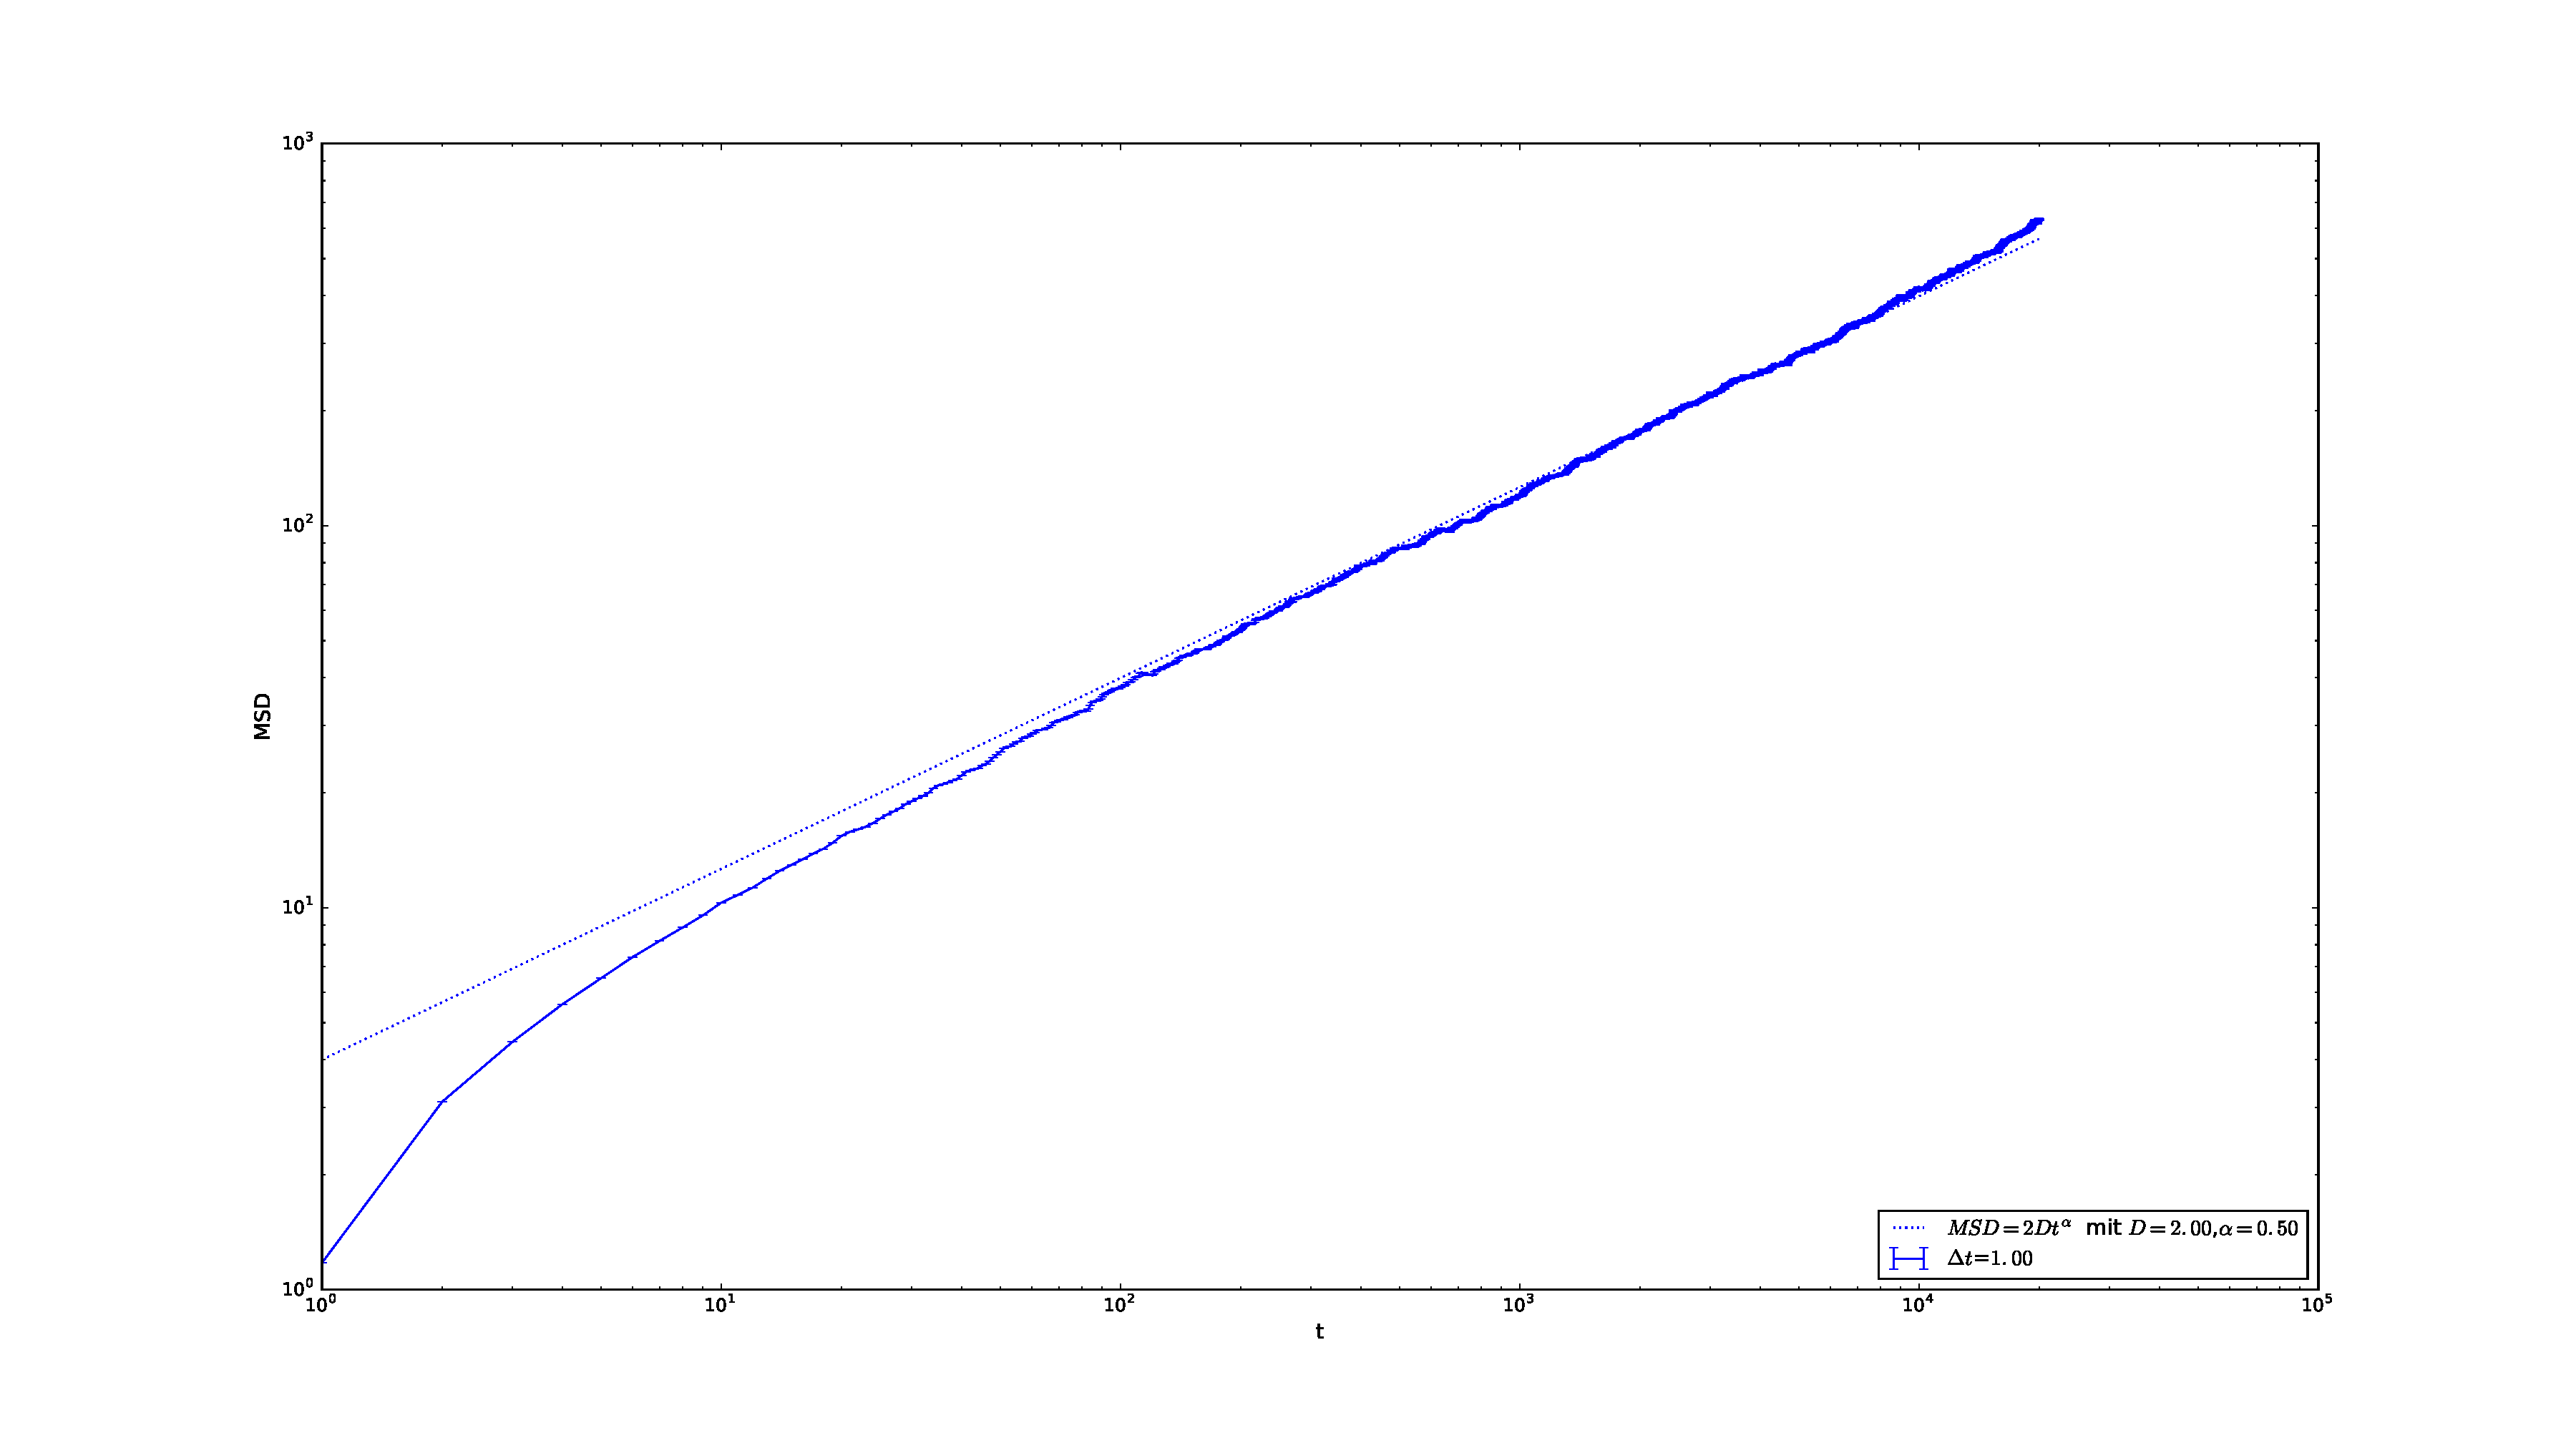
\includegraphics[width=\textwidth]{./msd_ensemble_4000particles_log.pdf}
\caption{Mean Square Displacement (Ensemble average of 4000 Trajectories)}
% msd_ensemble_4000particles_log.pdf: 0x0 pixel, -2147483648dpi, 0.00x0.00 cm, bb=
 \centering
\end{figure}

\begin{figure}[h]
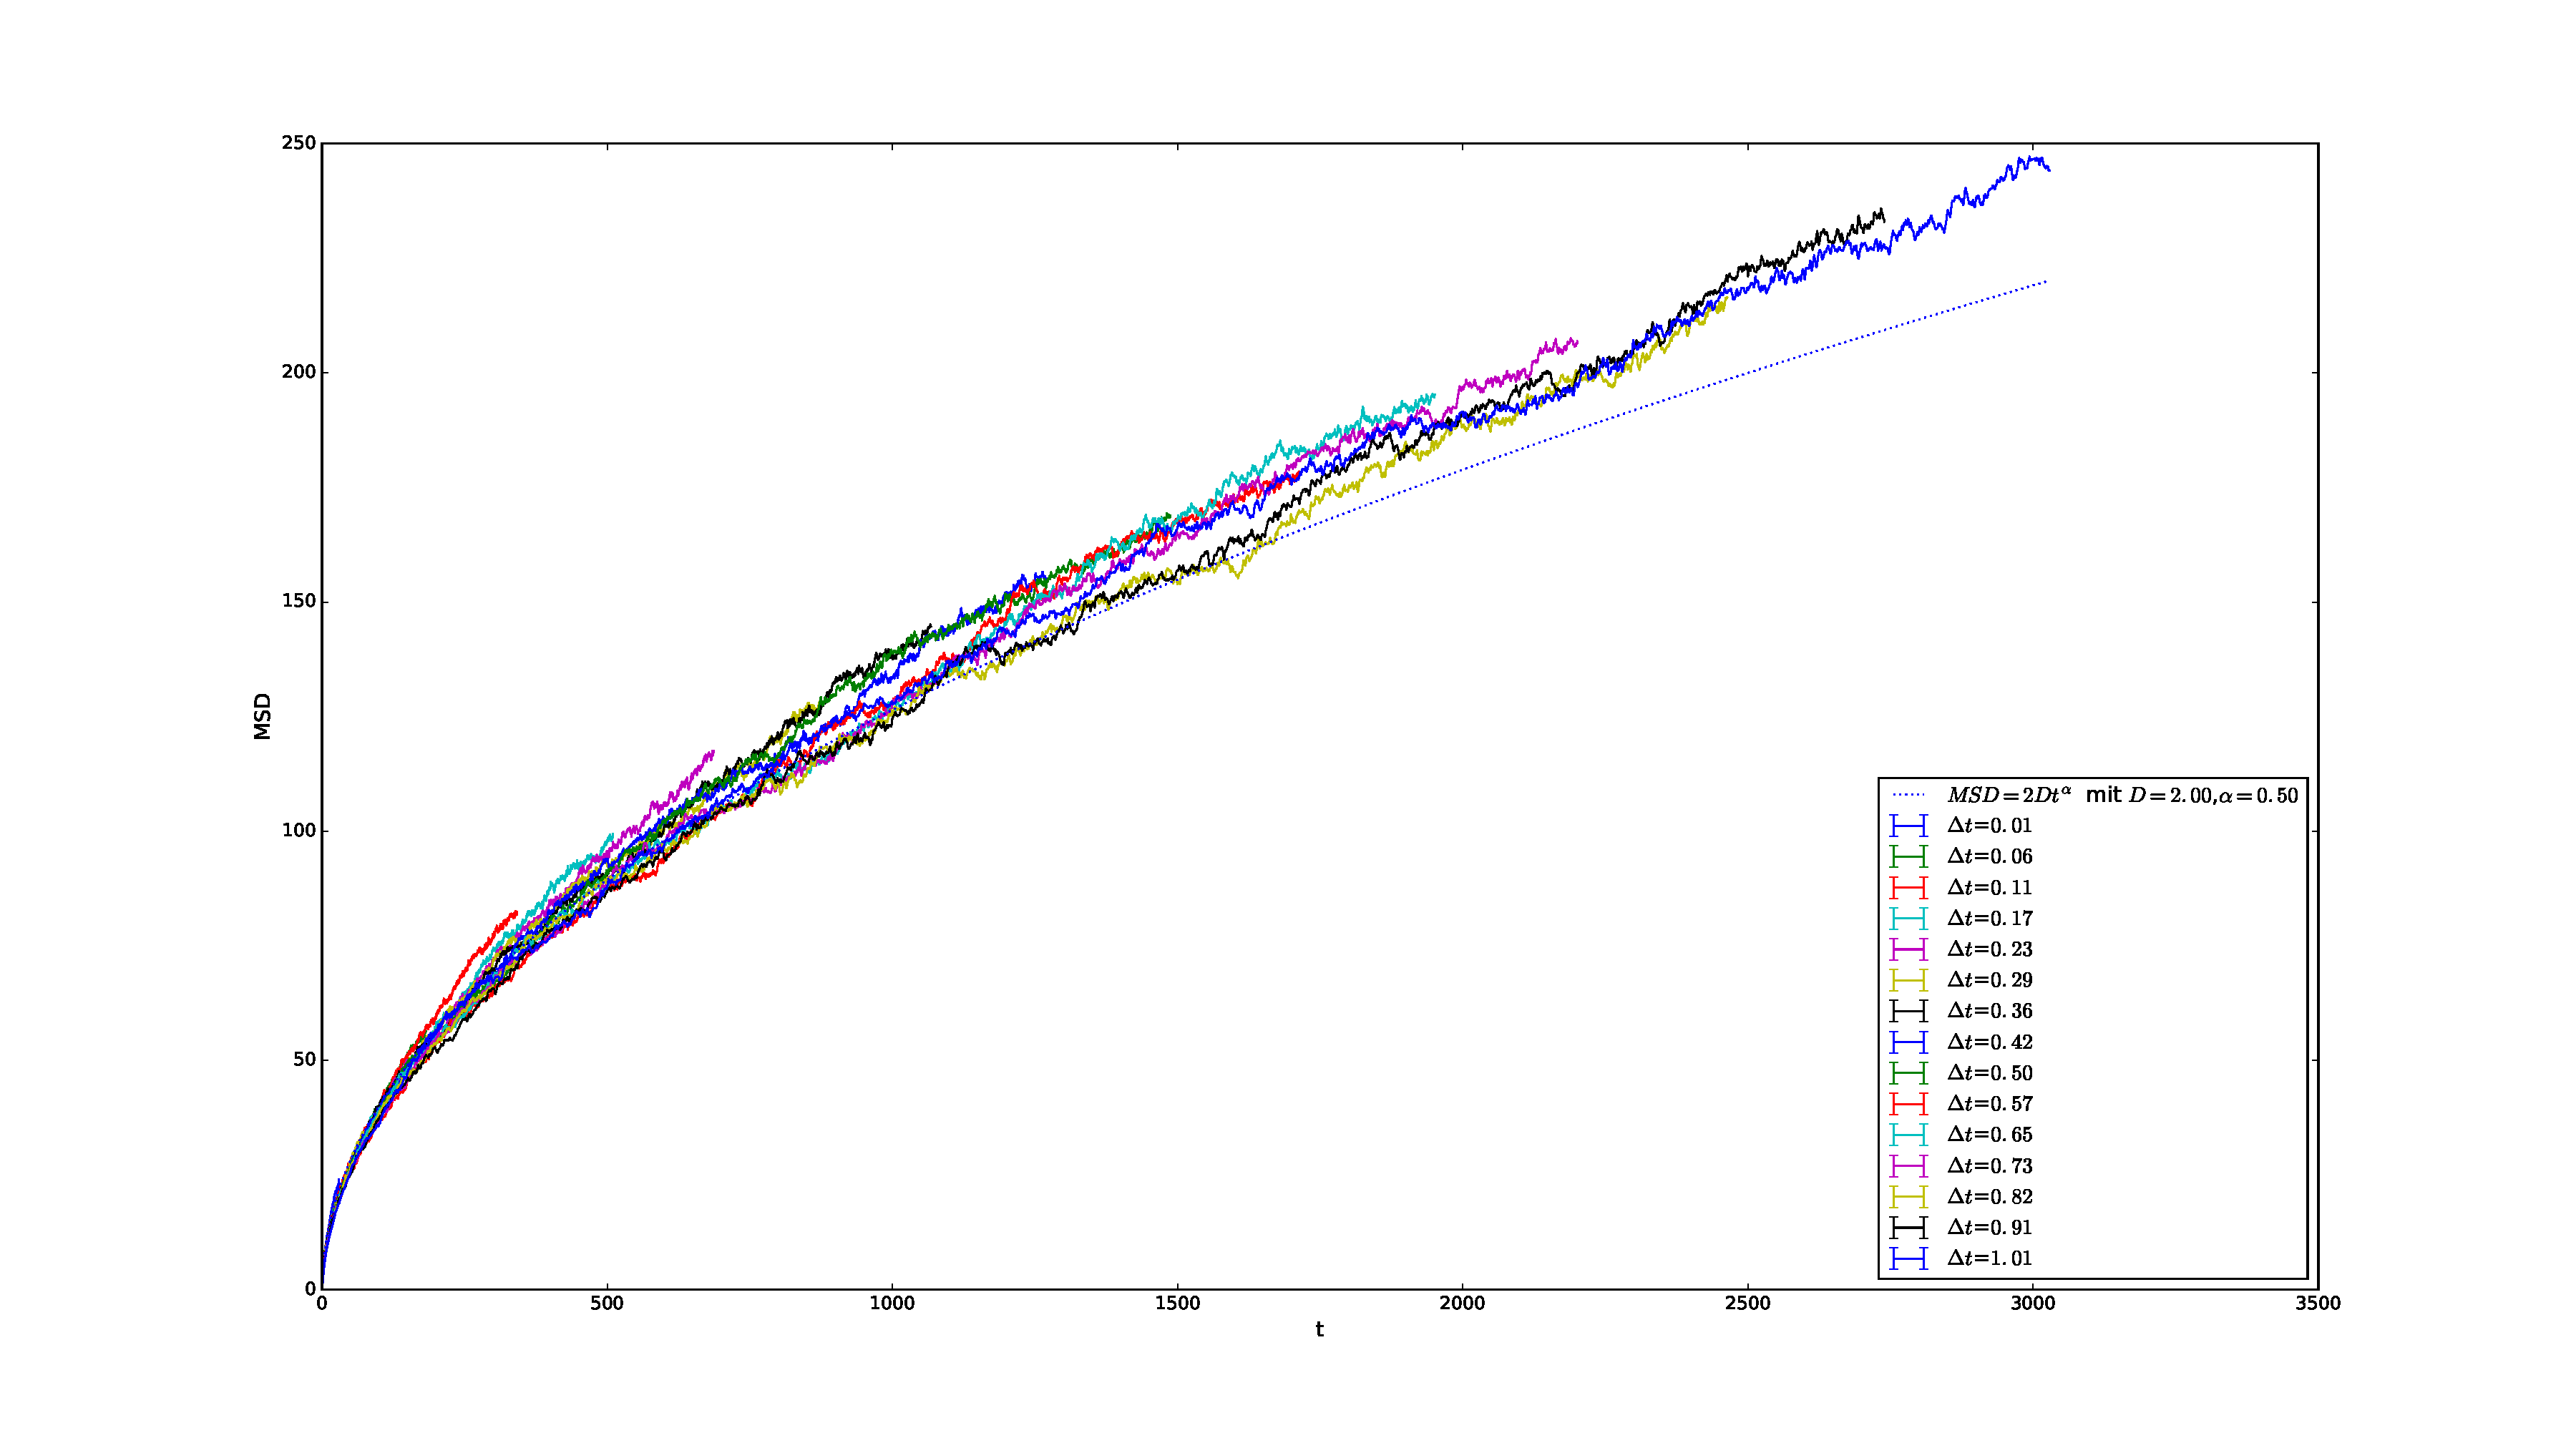
\includegraphics[width=\textwidth]{./msd_ensemble_dt_nostd_lin.pdf}
\caption{Mean Square Displacement (Ensemble average fpr different $\Delta t$)}
% msd_ensemble_4000particles_log.pdf: 0x0 pixel, -2147483648dpi, 0.00x0.00 cm, bb=
 \centering
\end{figure}

\begin{figure}[h]
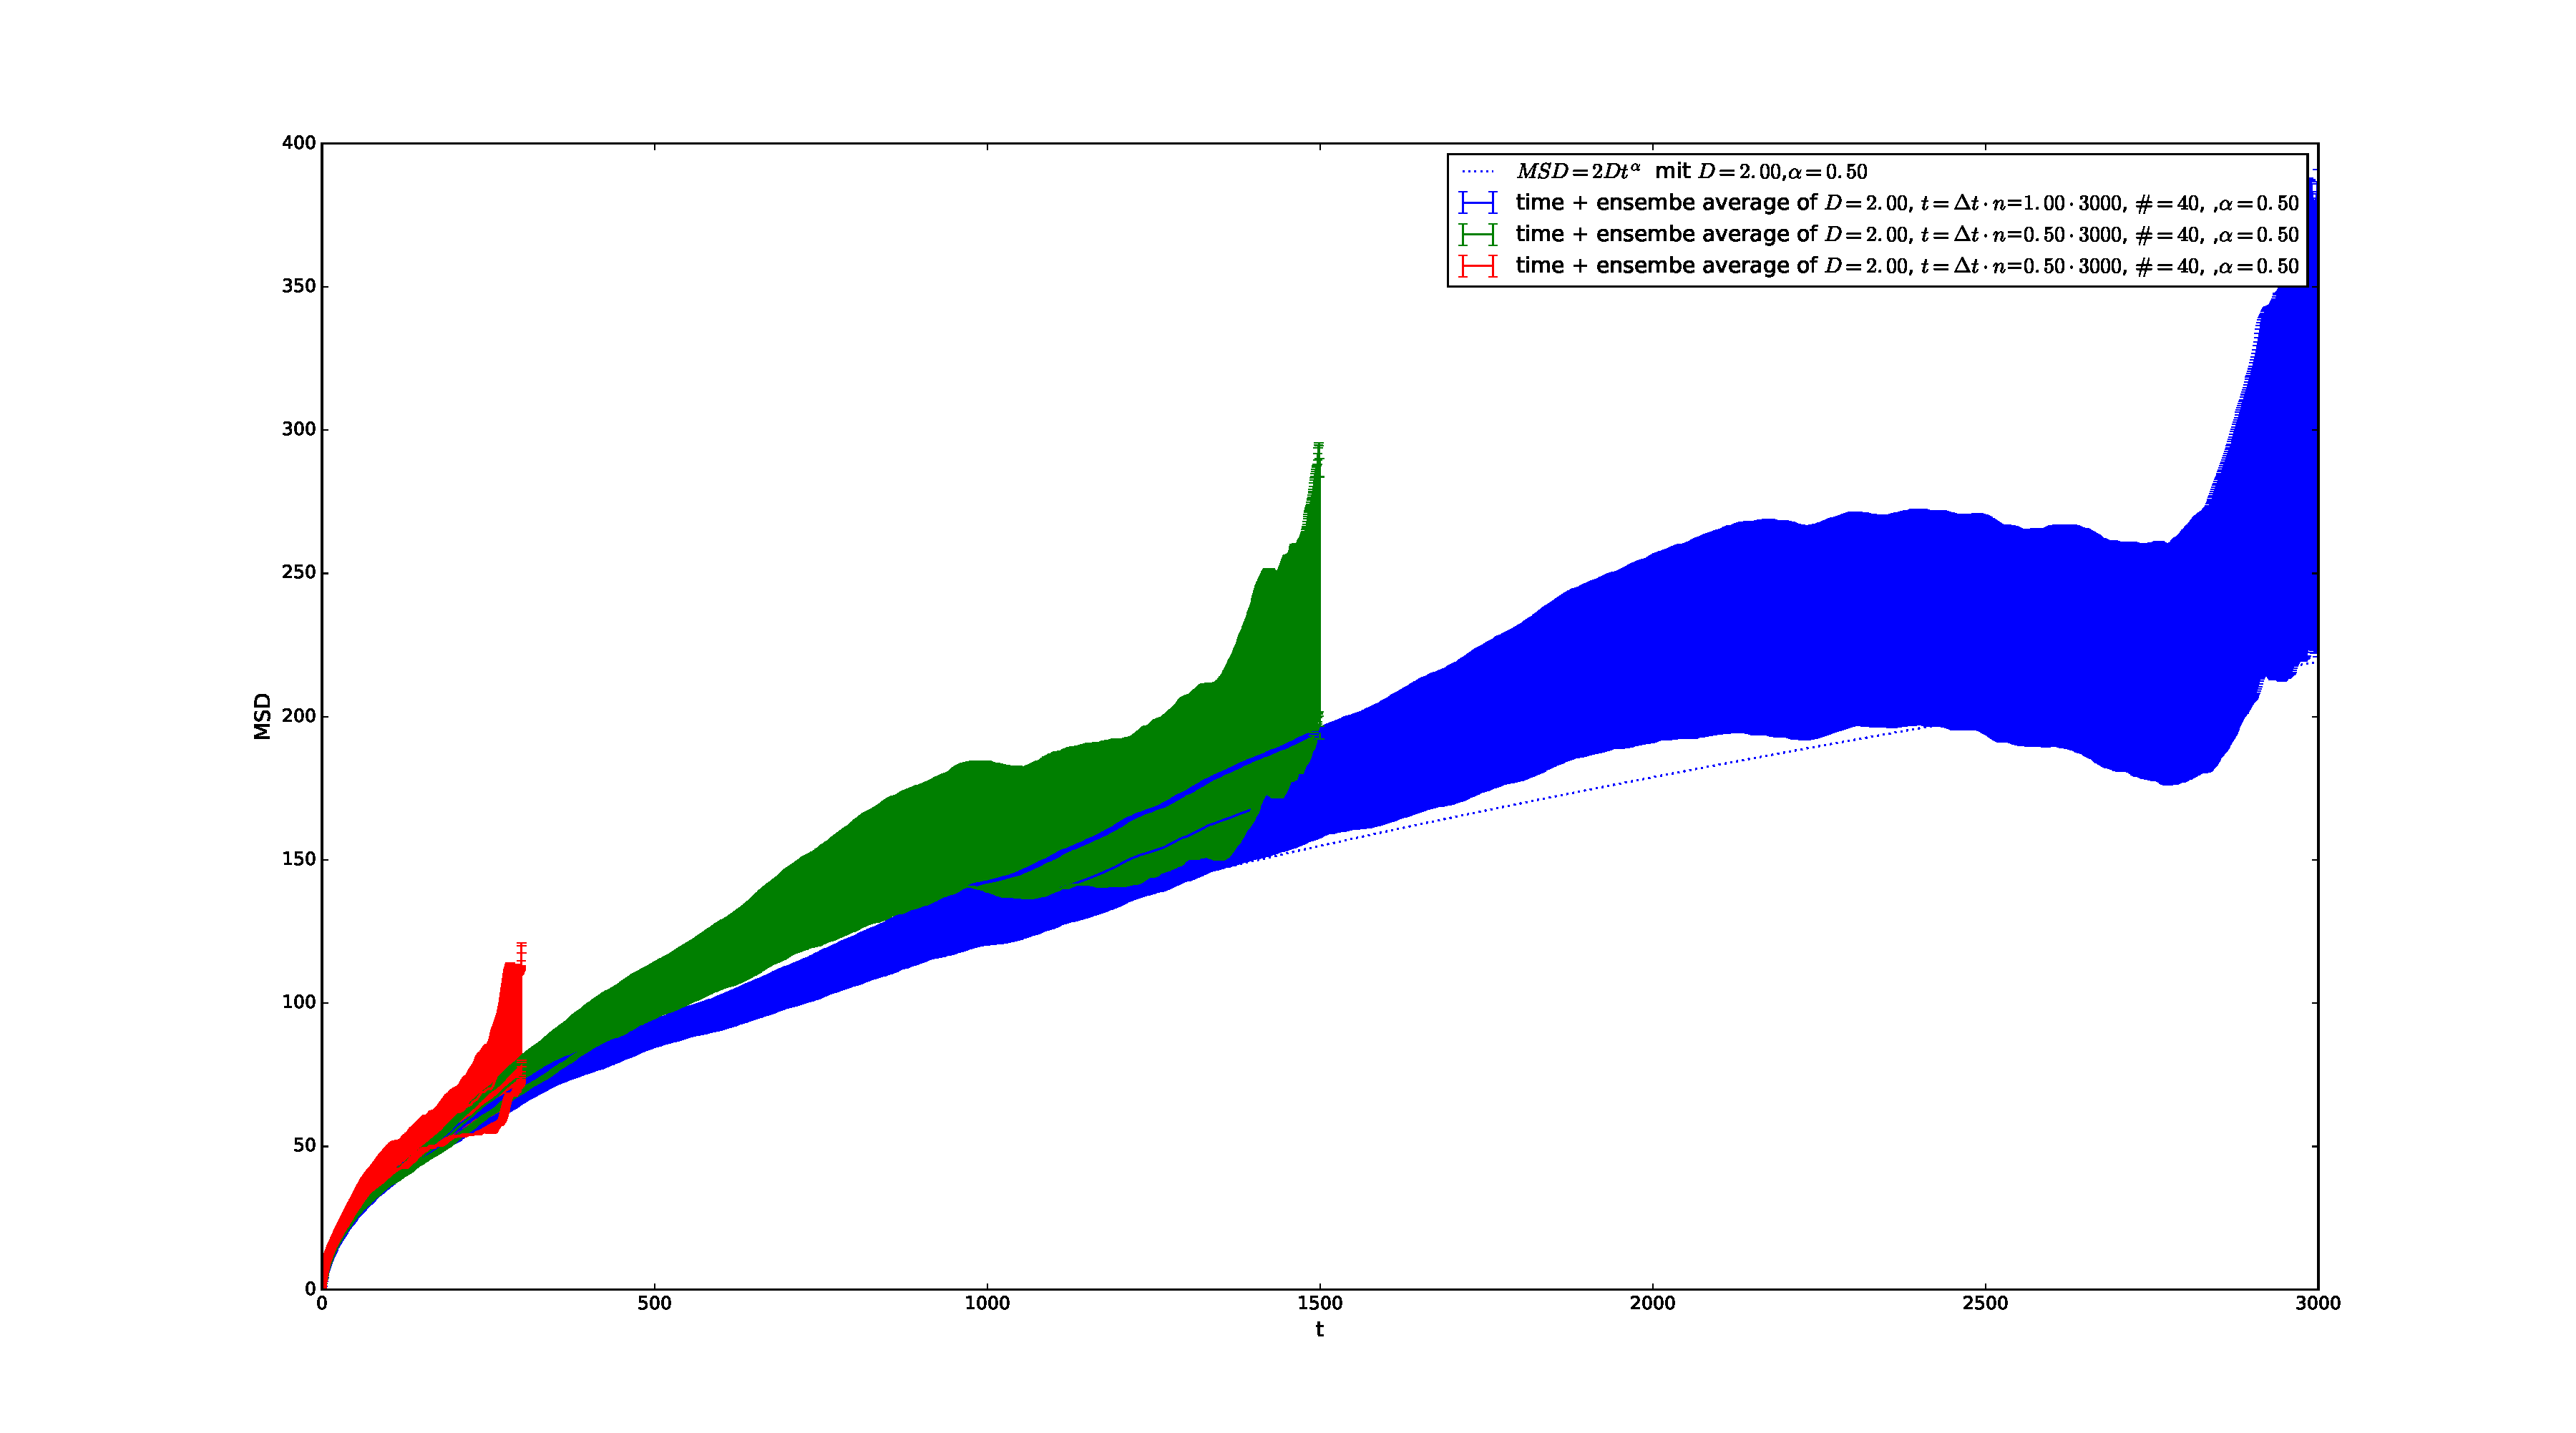
\includegraphics[width=\textwidth]{./msd_time_ensemble_dt_lin.pdf}
\caption{Mean Square Displacement (time and ensemble avarge for different $ \Delta t$ and with standard deviation of the Mean)}
% msd_ensemble_4000particles_log.pdf: 0x0 pixel, -2147483648dpi, 0.00x0.00 cm, bb=
 \centering
\end{figure}

\begin{figure}[h]
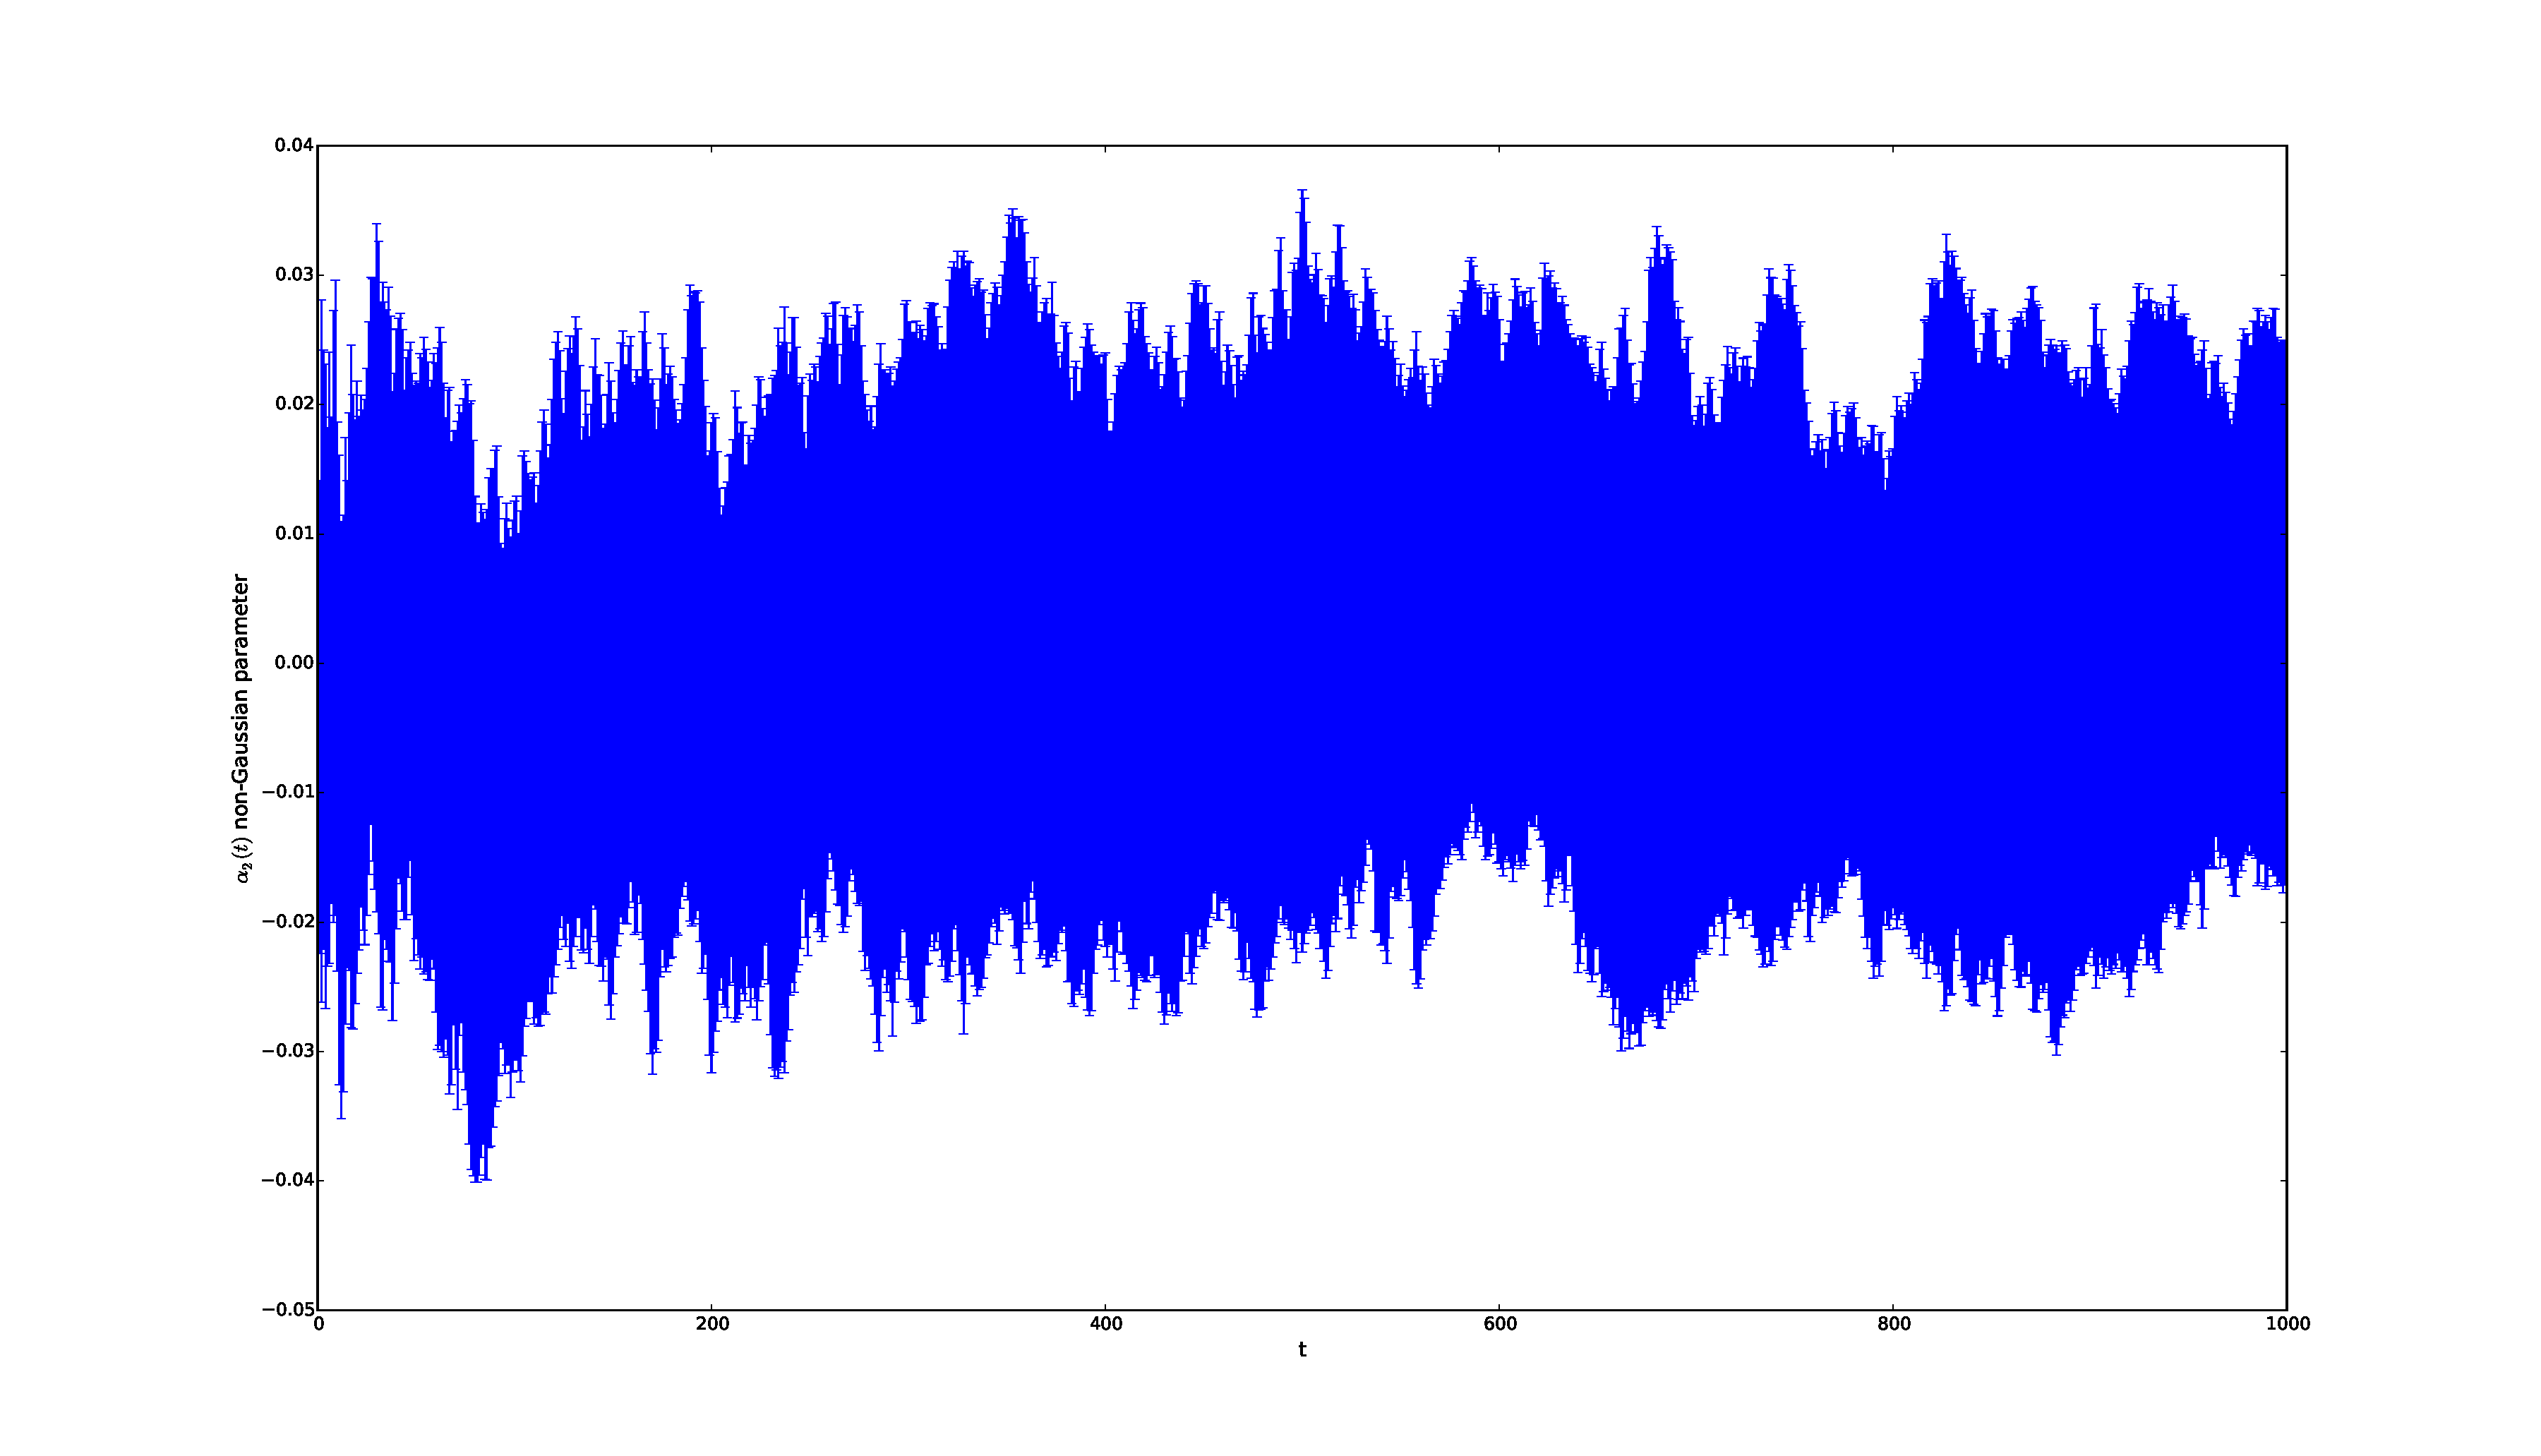
\includegraphics[width=\textwidth]{./non_gaussian_D=2_t=1001_dt=1_alpha=05particles_5000_std01.pdf}
\caption{Non-gaussian parameter of $\alpha=0.5$ , $ D=2 $ and 5000 trajectories ensemble.}
% msd_ensemble_4000particles_log.pdf: 0x0 pixel, -2147483648dpi, 0.00x0.00 cm, bb=
 \centering
\end{figure}

\begin{figure}[h]
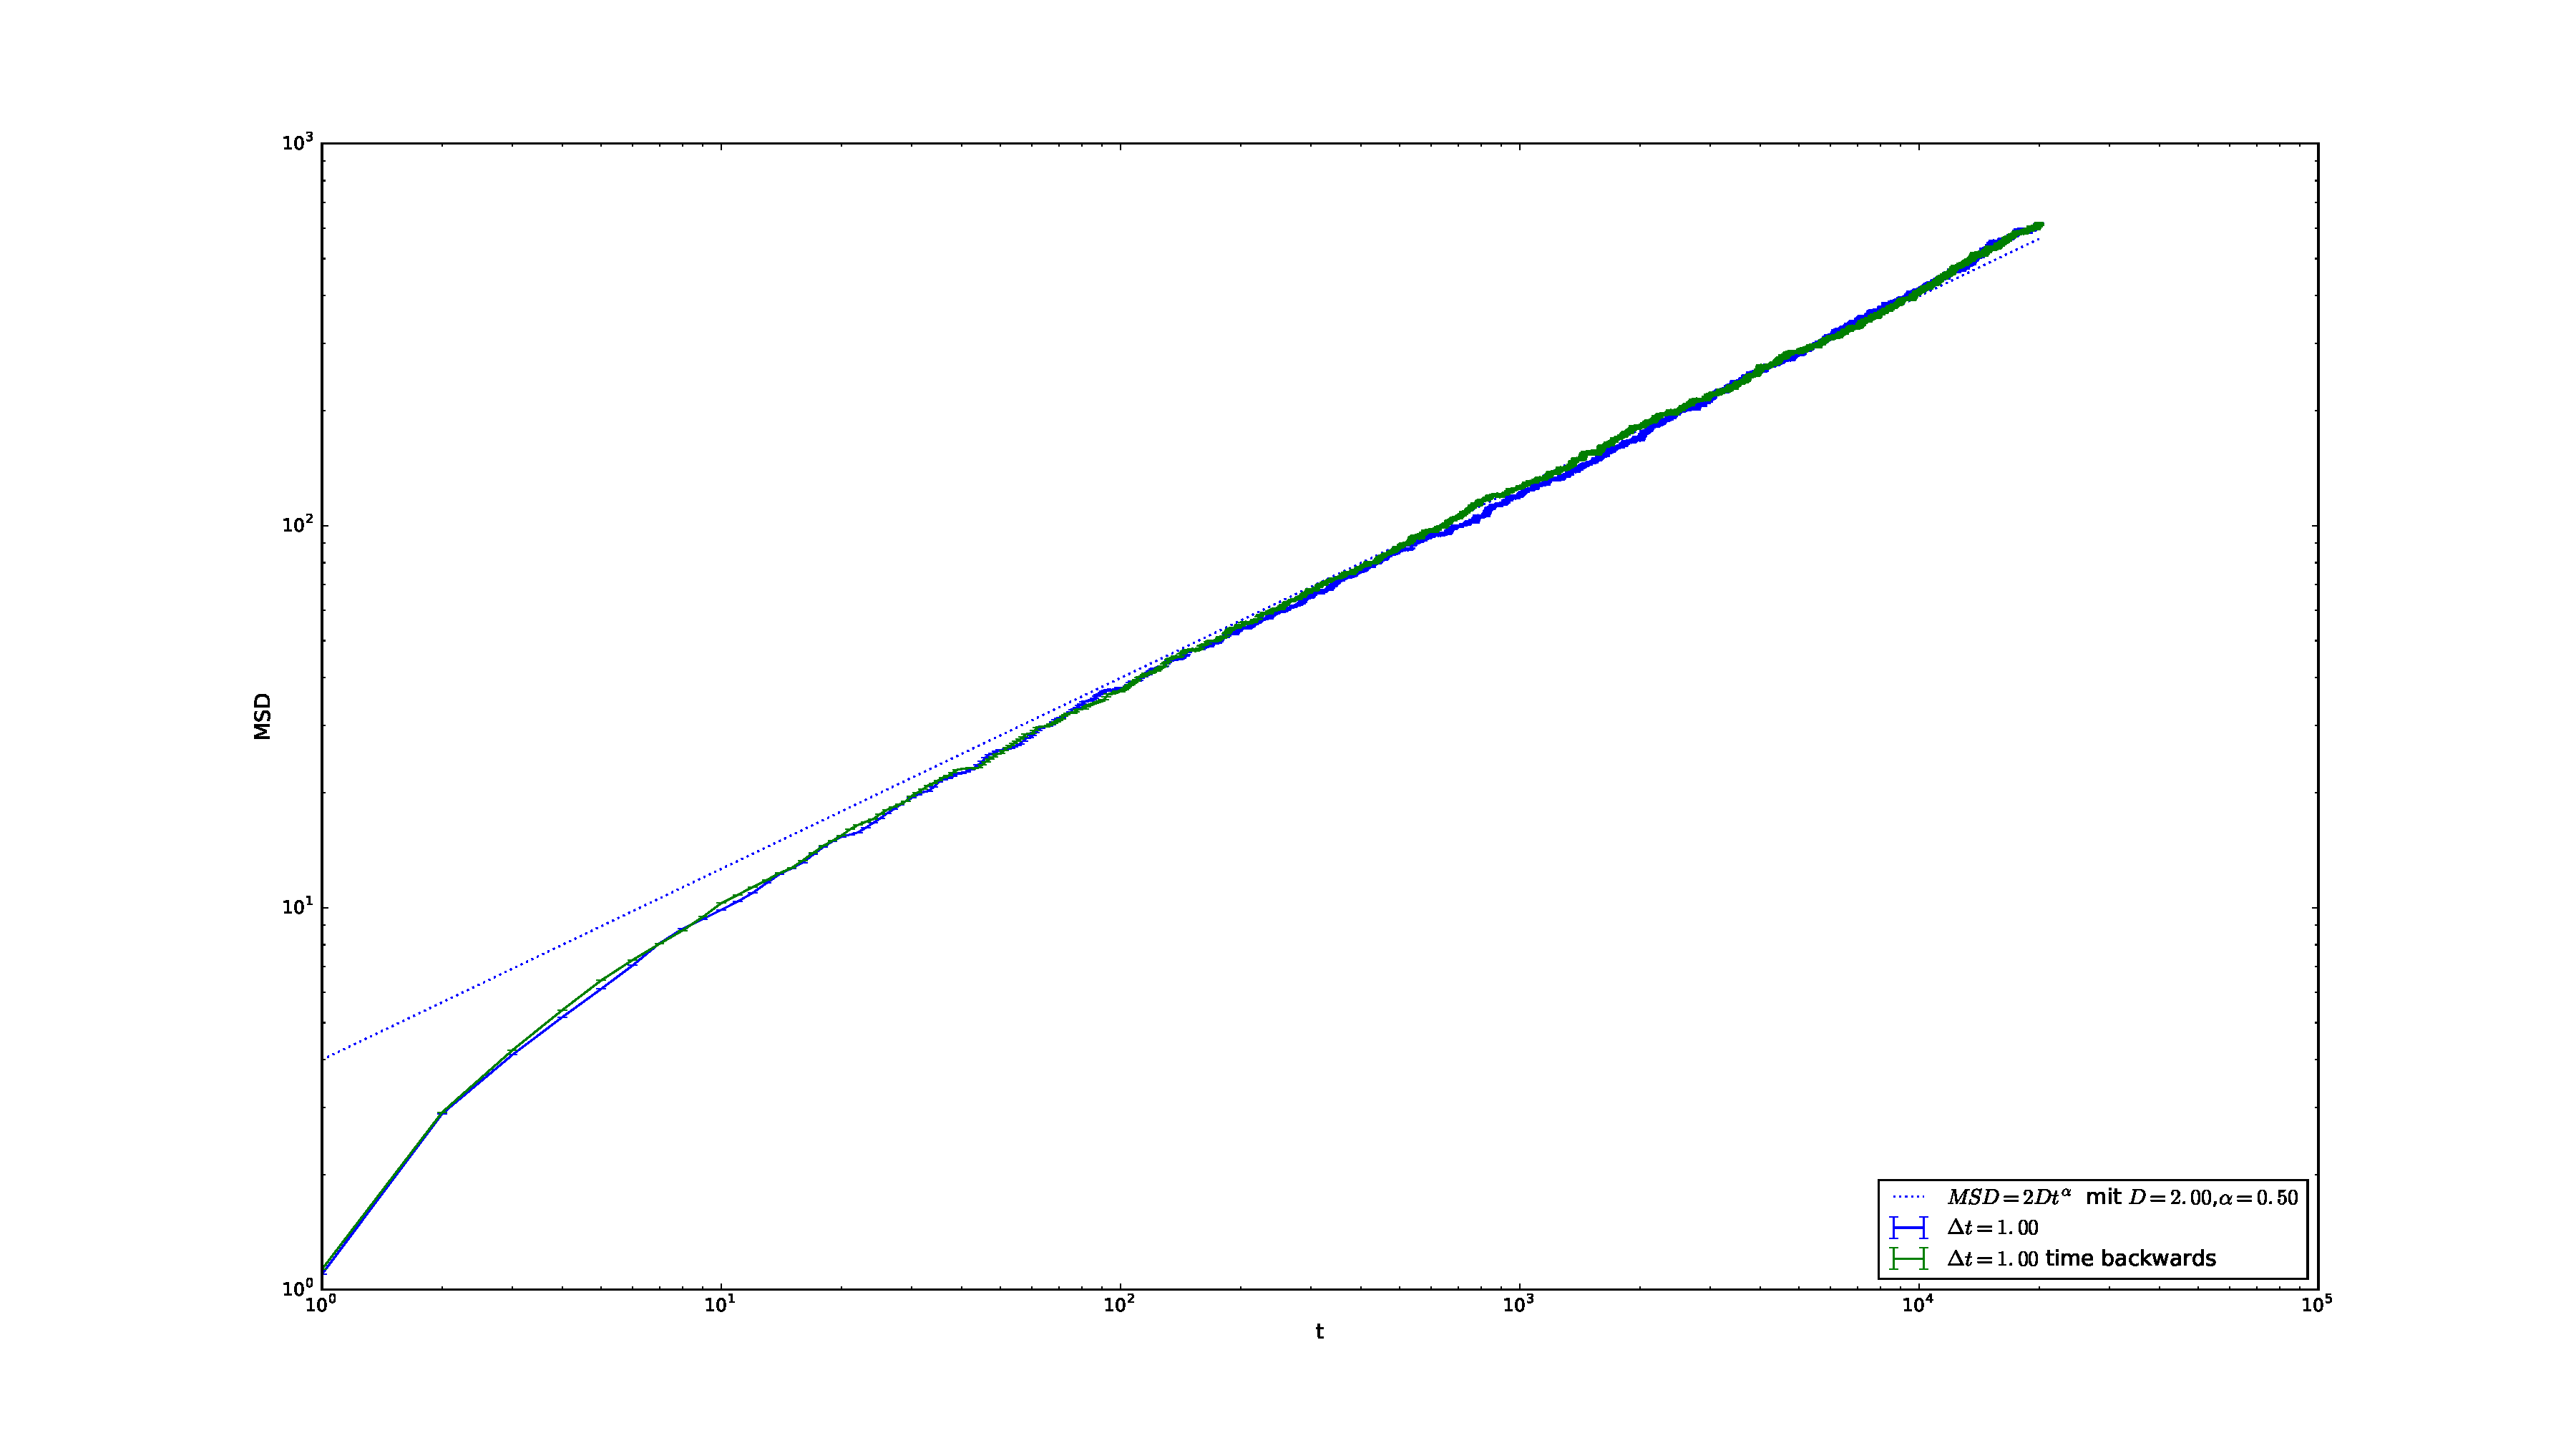
\includegraphics[width=\textwidth]{./msd_ensemble_t_inverted.pdf}
\caption{Non-gaussian parameter of $\alpha=0.5$ , $ D=2 $ and 5000 trajectories ensemble.}
% msd_ensemble_4000particles_log.pdf: 0x0 pixel, -2147483648dpi, 0.00x0.00 cm, bb=
 \centering
\end{figure}

\begin{figure}[h]
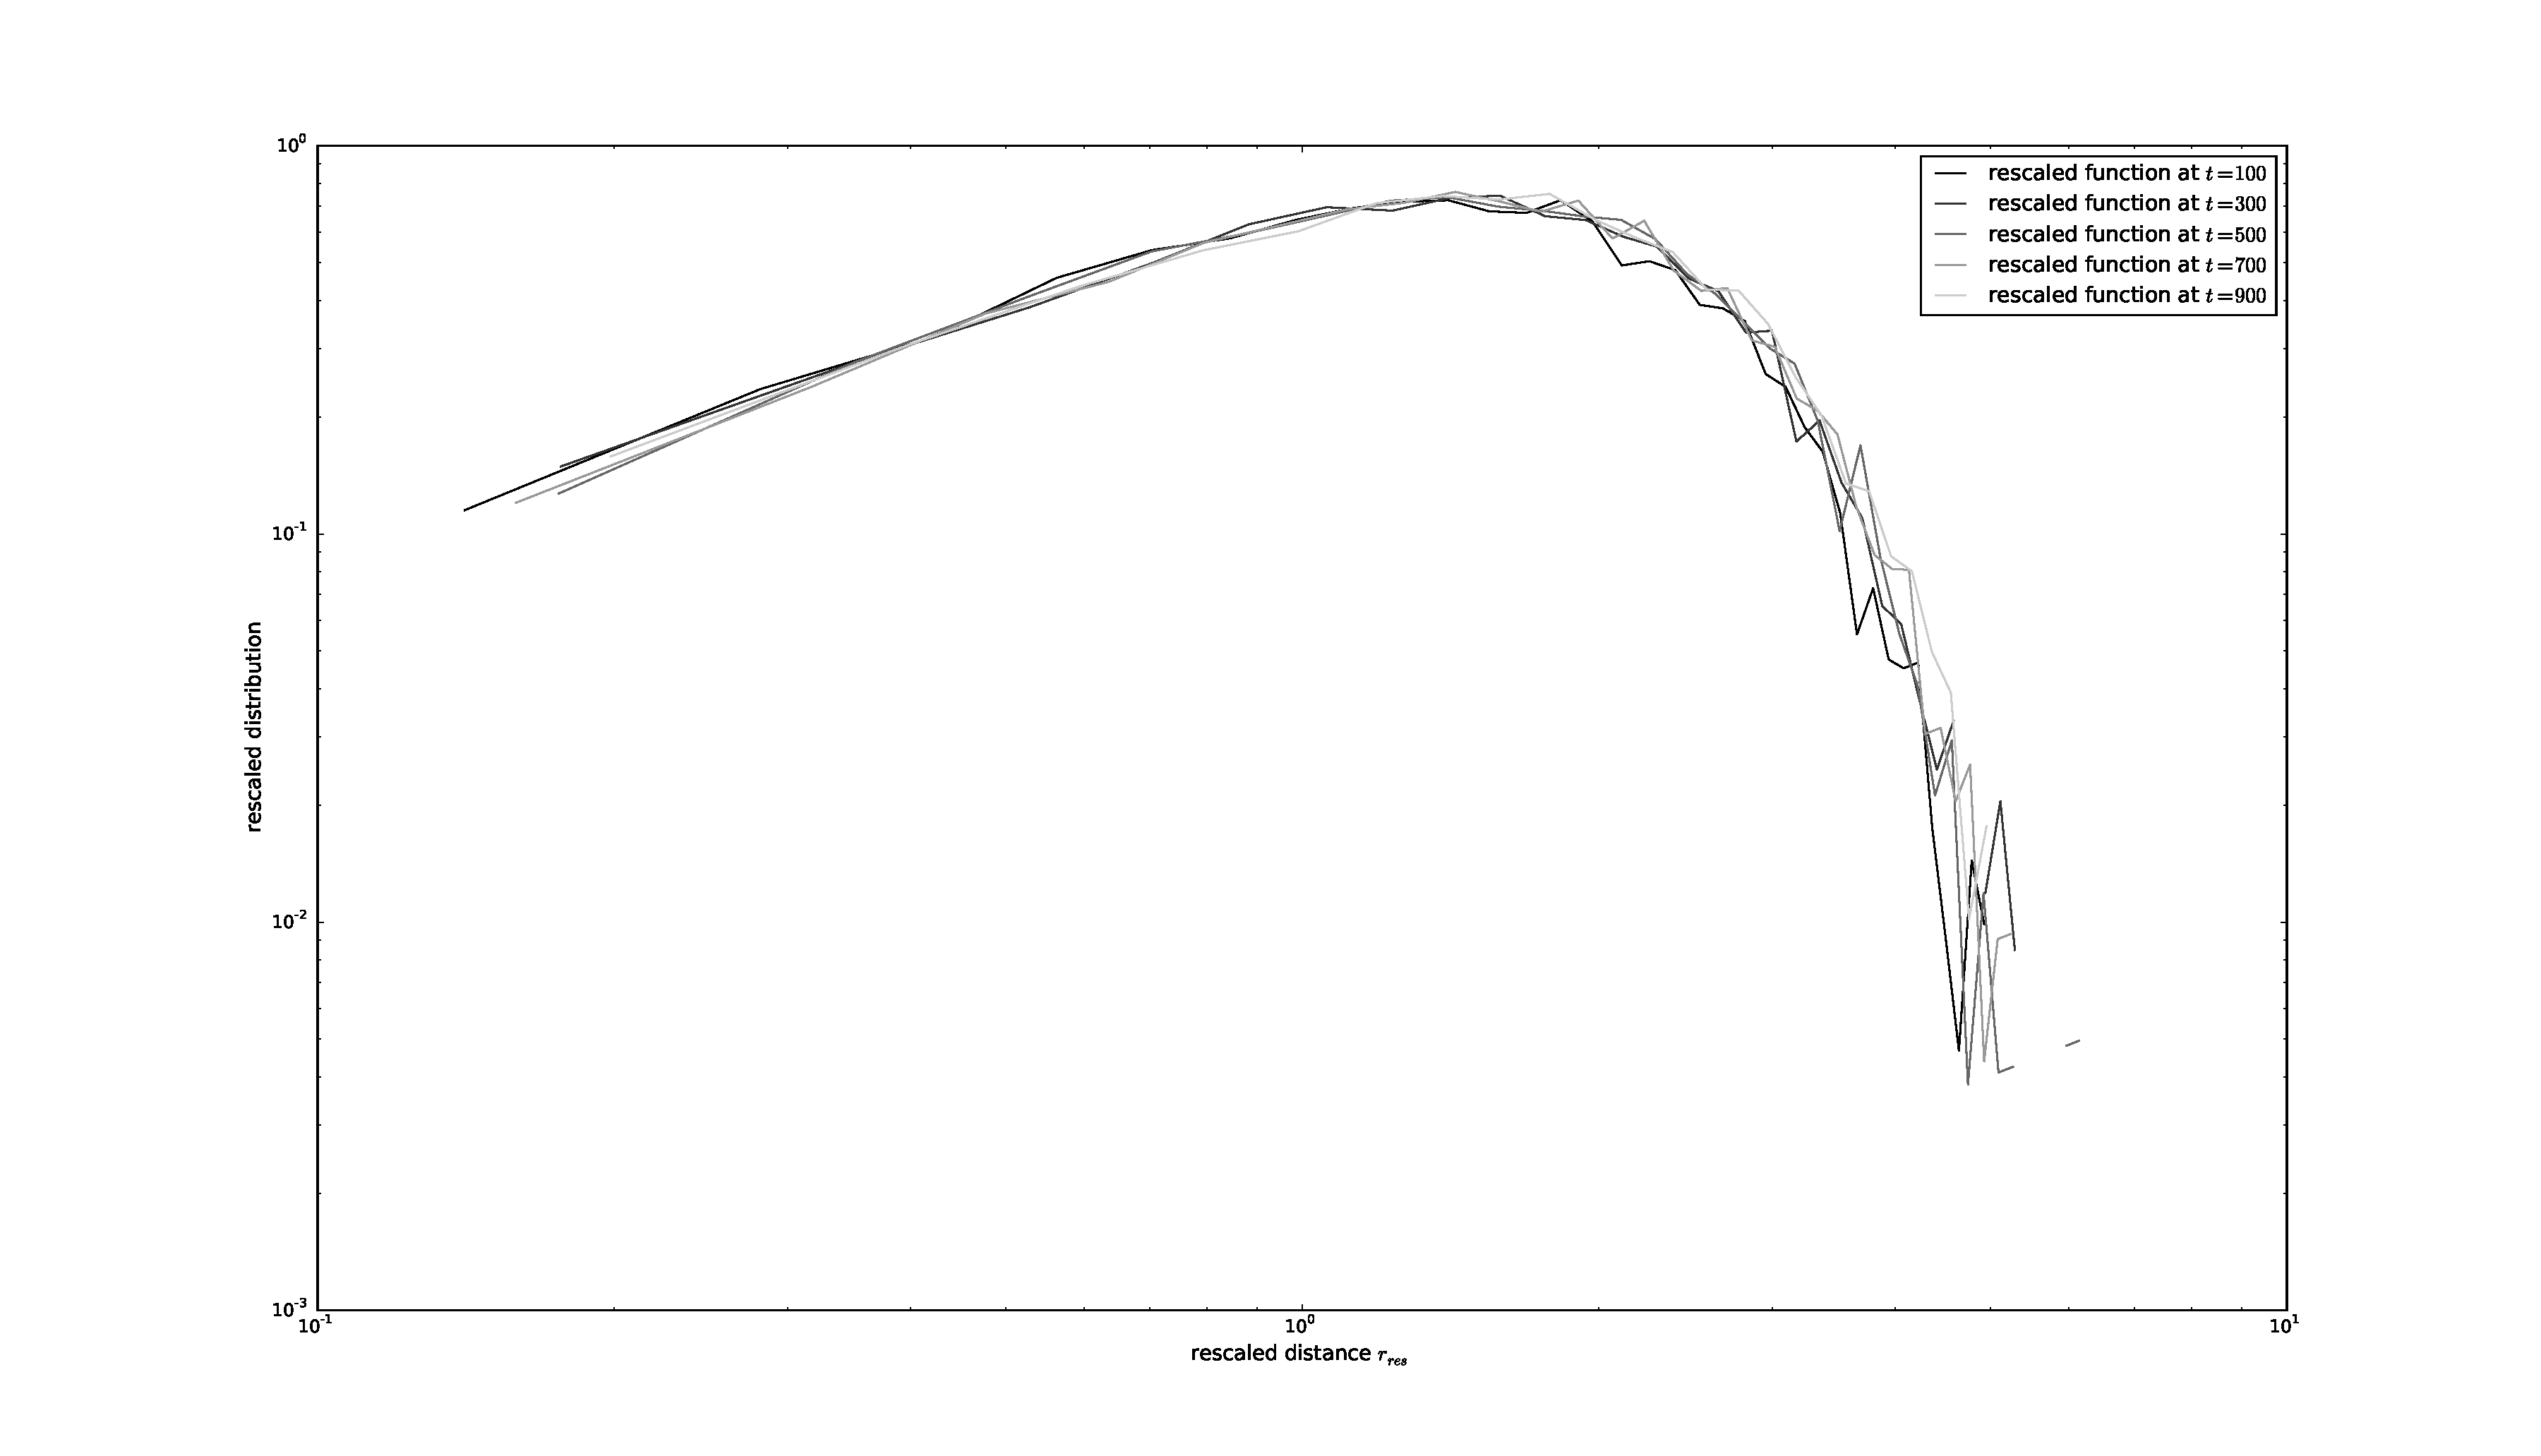
\includegraphics[width=\textwidth]{./rescaled_function.pdf}
\caption{rescaled function for different times}
% msd_ensemble_4000particles_log.pdf: 0x0 pixel, -2147483648dpi, 0.00x0.00 cm, bb=
 \centering
\end{figure}

\begin{figure}[h]
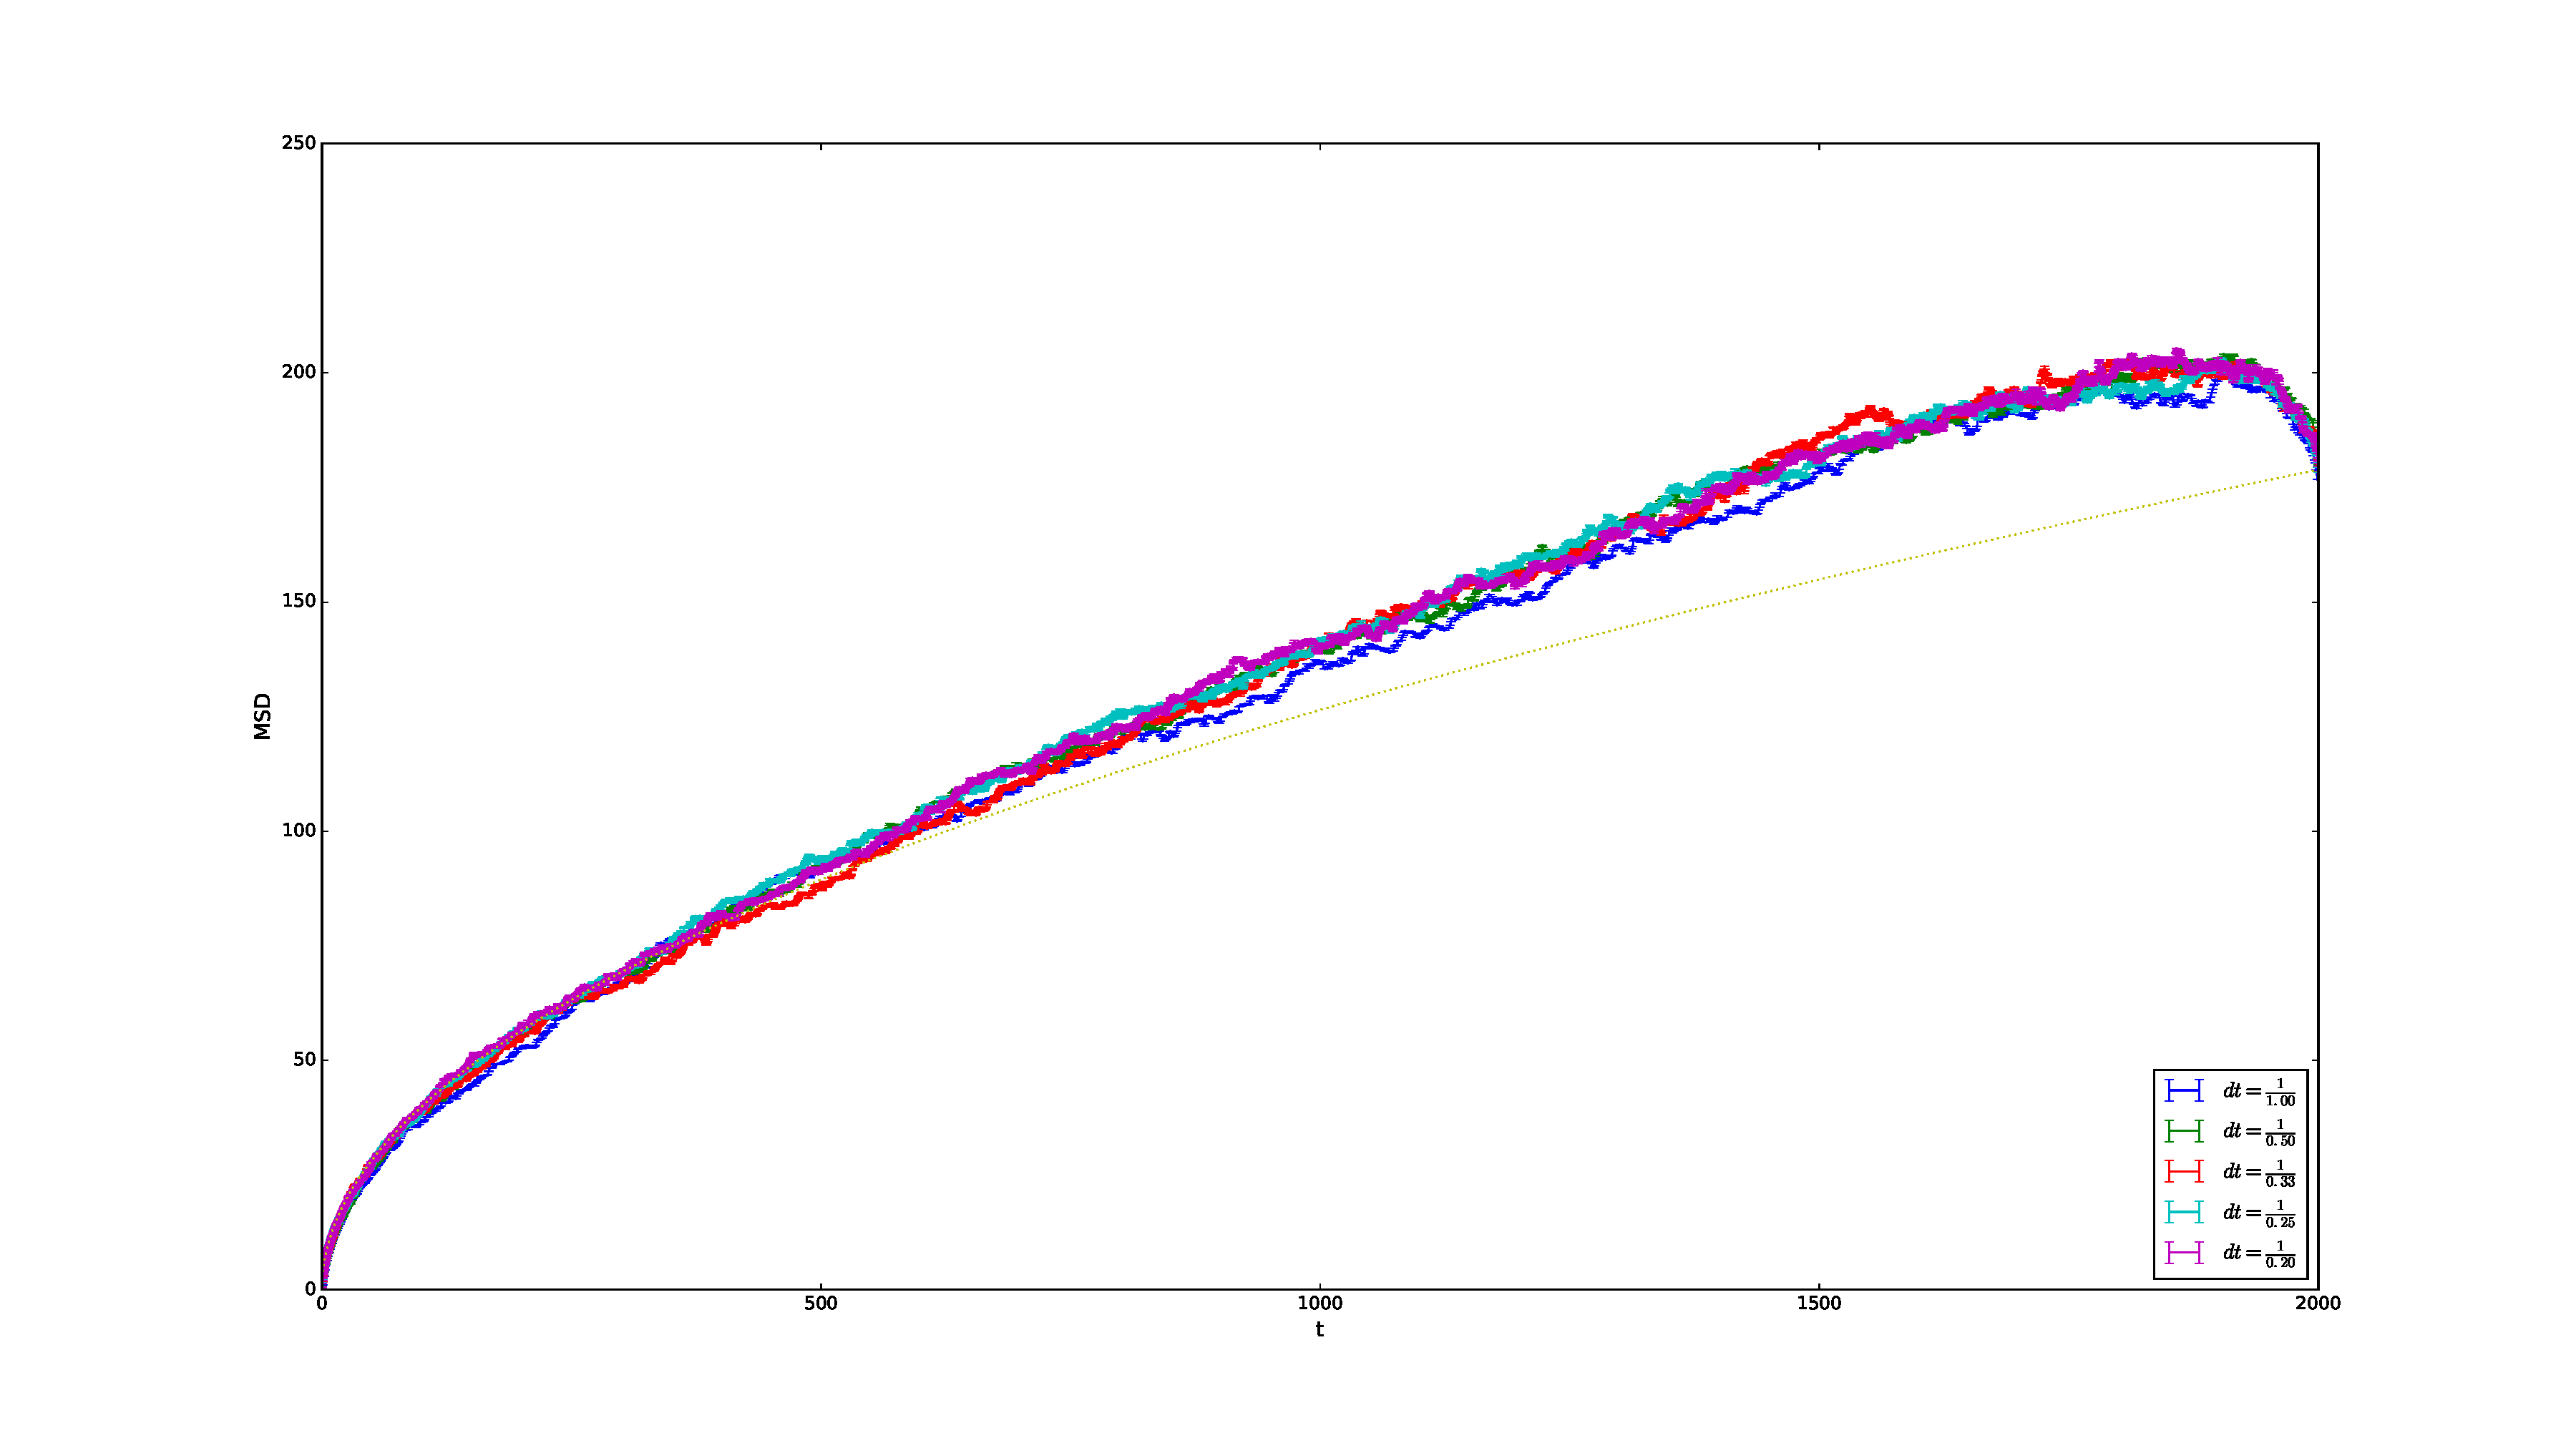
\includegraphics[width=\textwidth]{./dt_variert_bei_factor_1_lin.pdf}
\caption{variere dt bei gleichem Faktor 1}
% msd_ensemble_4000particles_log.pdf: 0x0 pixel, -2147483648dpi, 0.00x0.00 cm, bb=
 \centering
\end{figure}

\begin{figure}[h]
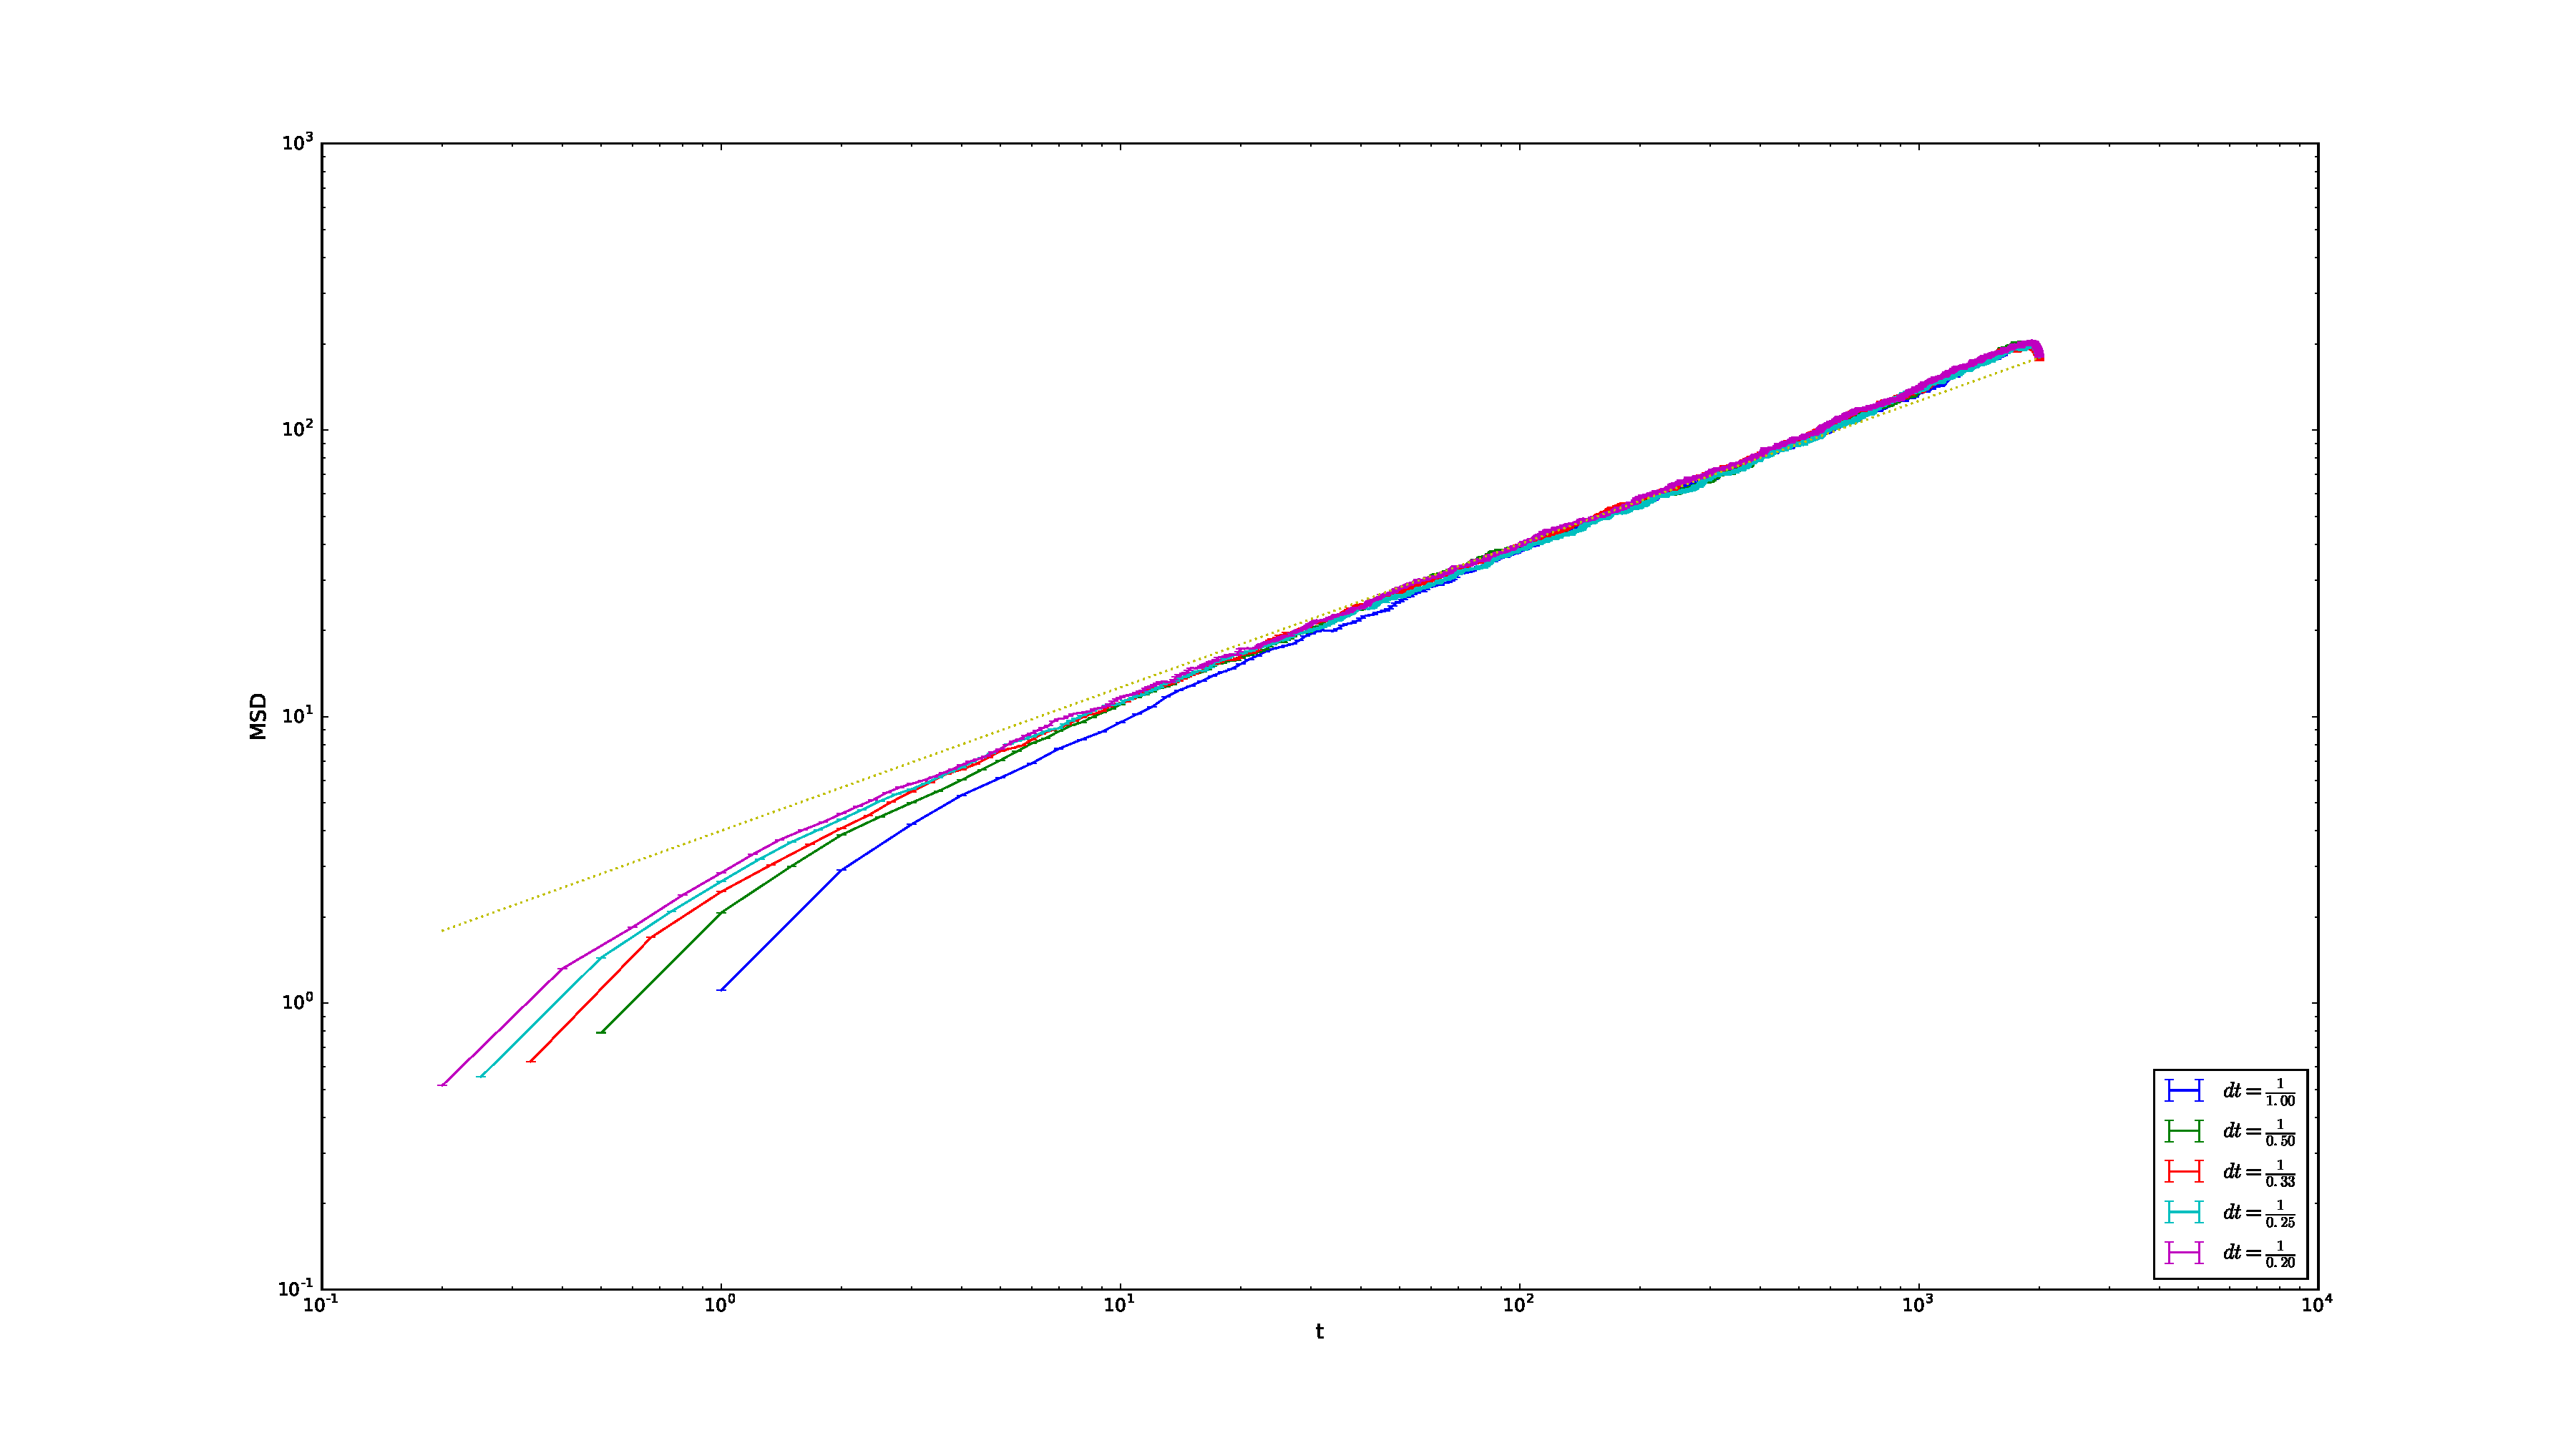
\includegraphics[width=\textwidth]{./dt_variert_bei_factor_1_log.pdf}
\caption{variere dt bei gleichem Faktor 1, logarithmisch}
% msd_ensemble_4000particles_log.pdf: 0x0 pixel, -2147483648dpi, 0.00x0.00 cm, bb=
 \centering
\end{figure}

\begin{figure}[h]
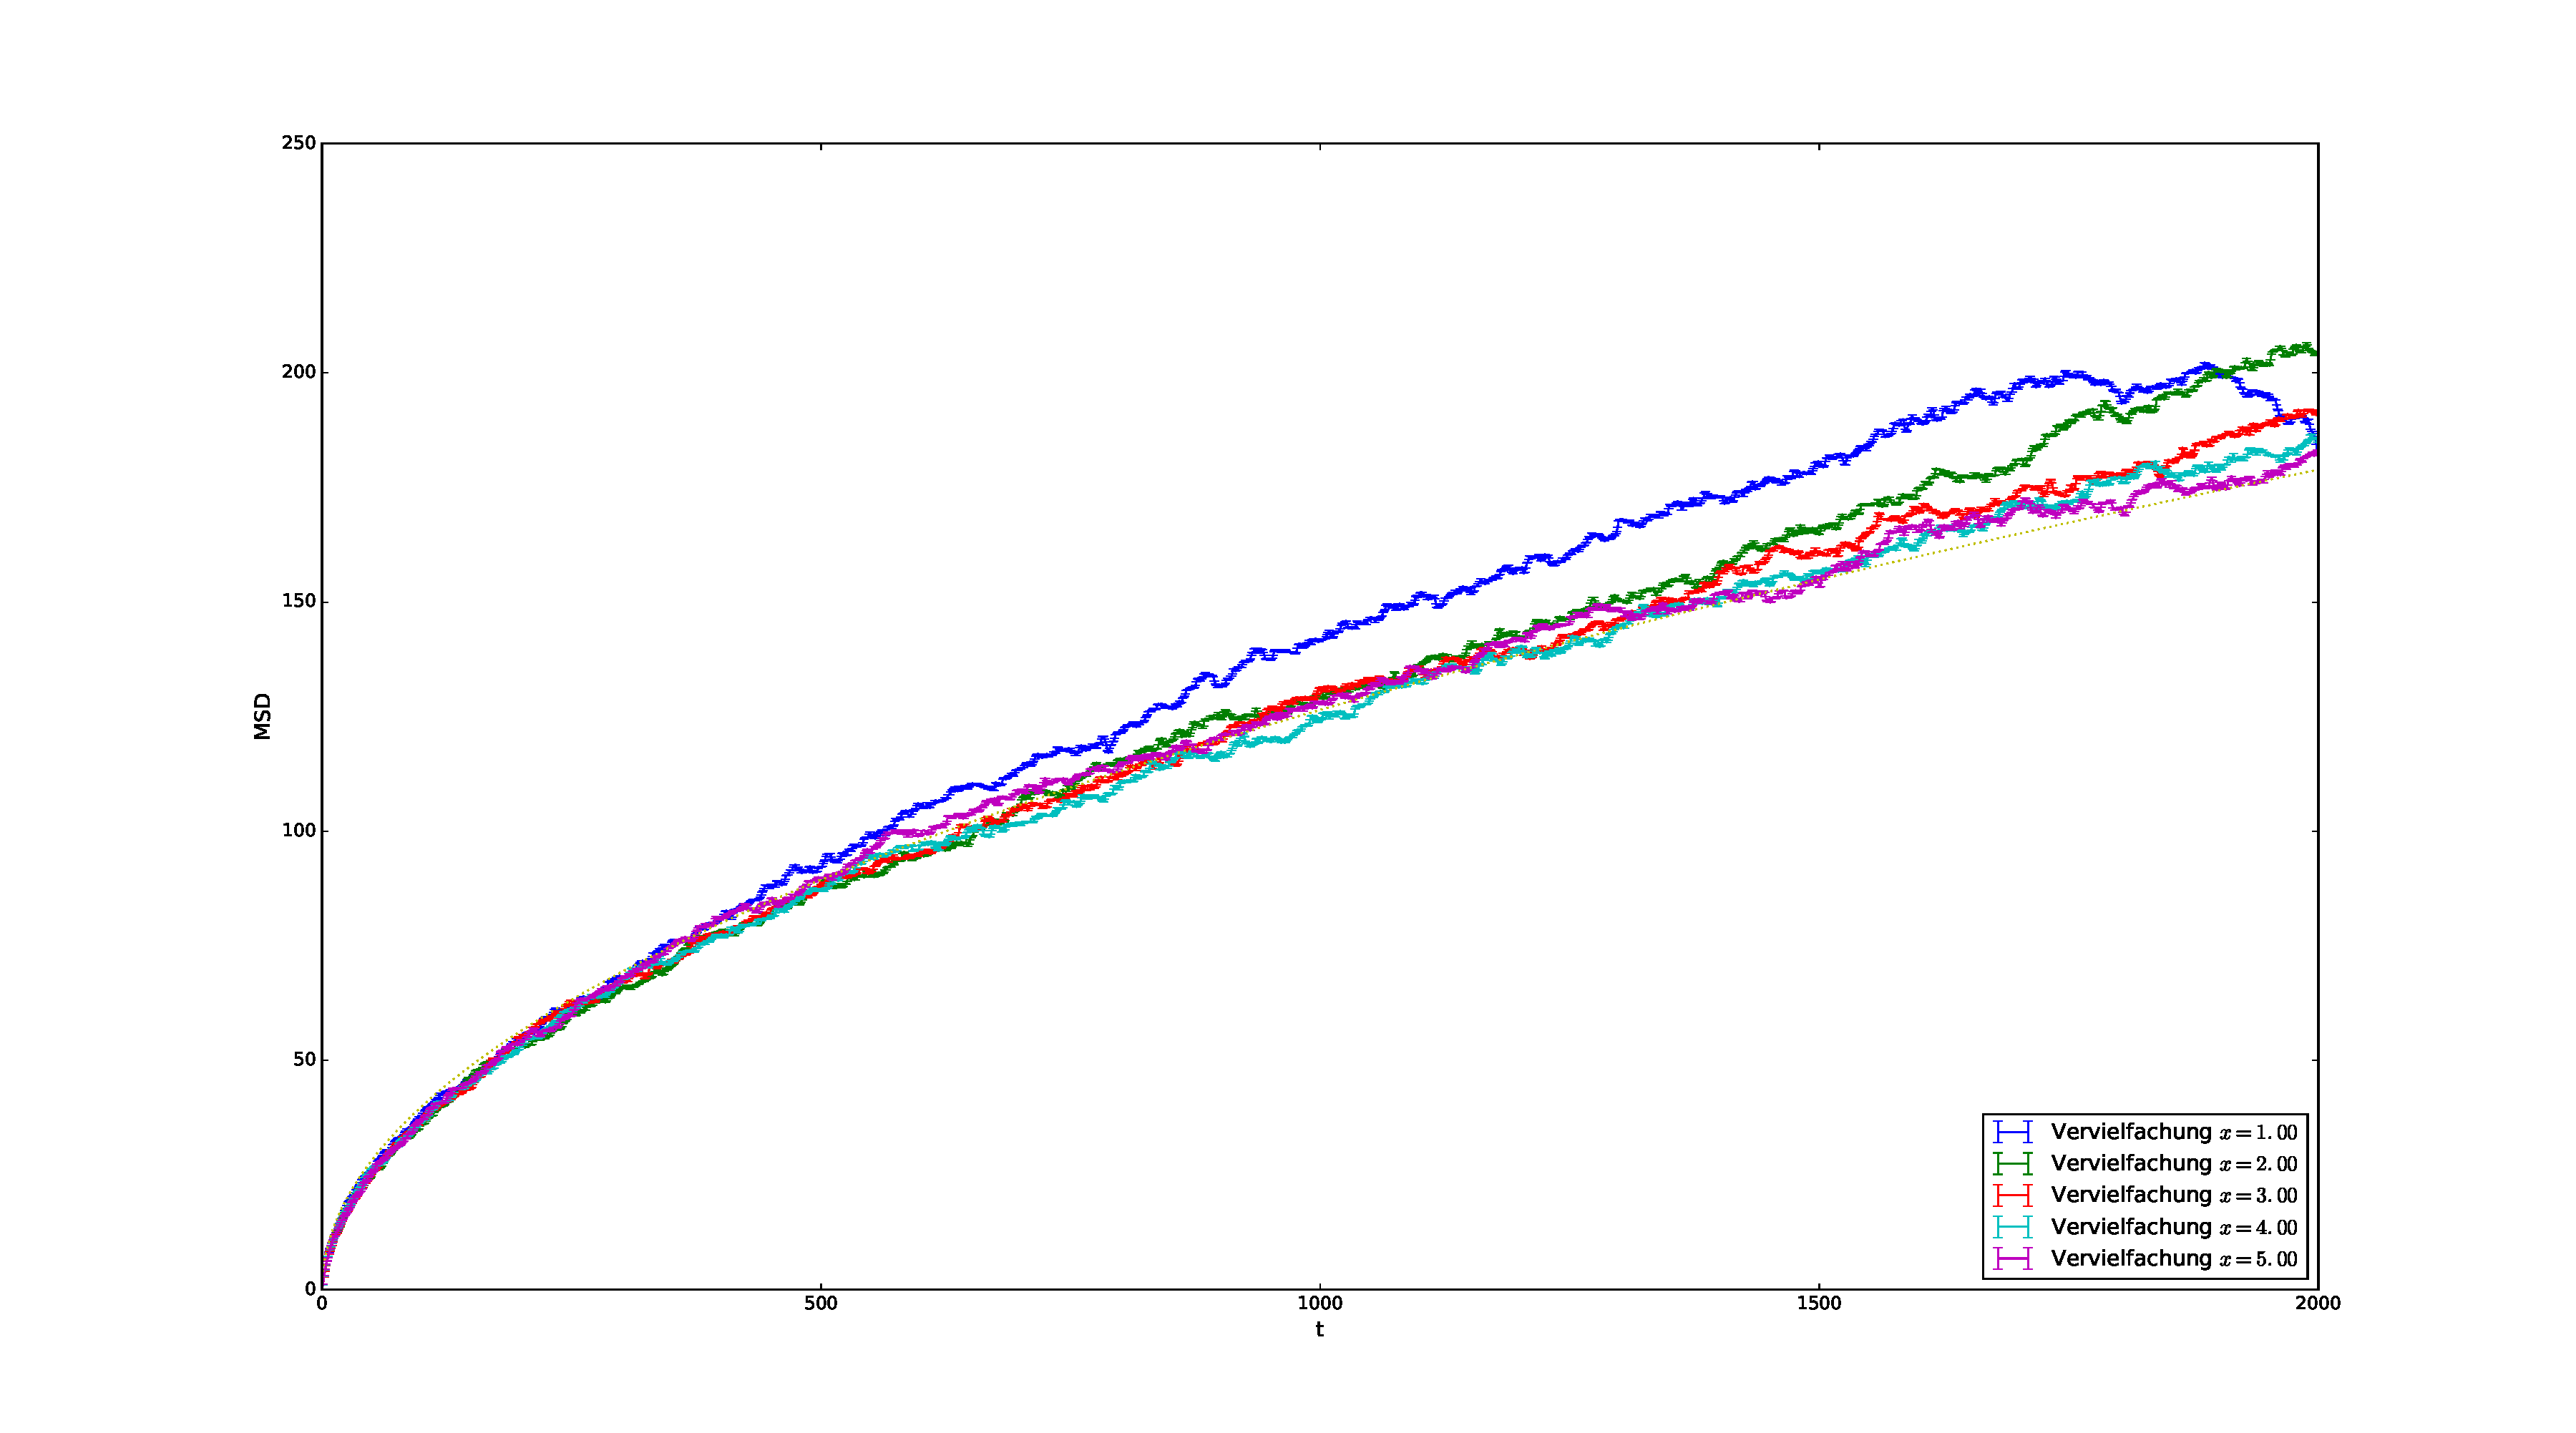
\includegraphics[width=\textwidth]{./faktor_variert_bei_dt_1_lin.pdf}
\caption{variere Faktor bei gleichem dt}
% msd_ensemble_4000particles_log.pdf: 0x0 pixel, -2147483648dpi, 0.00x0.00 cm, bb=
 \centering
\end{figure}

\begin{figure}[h]
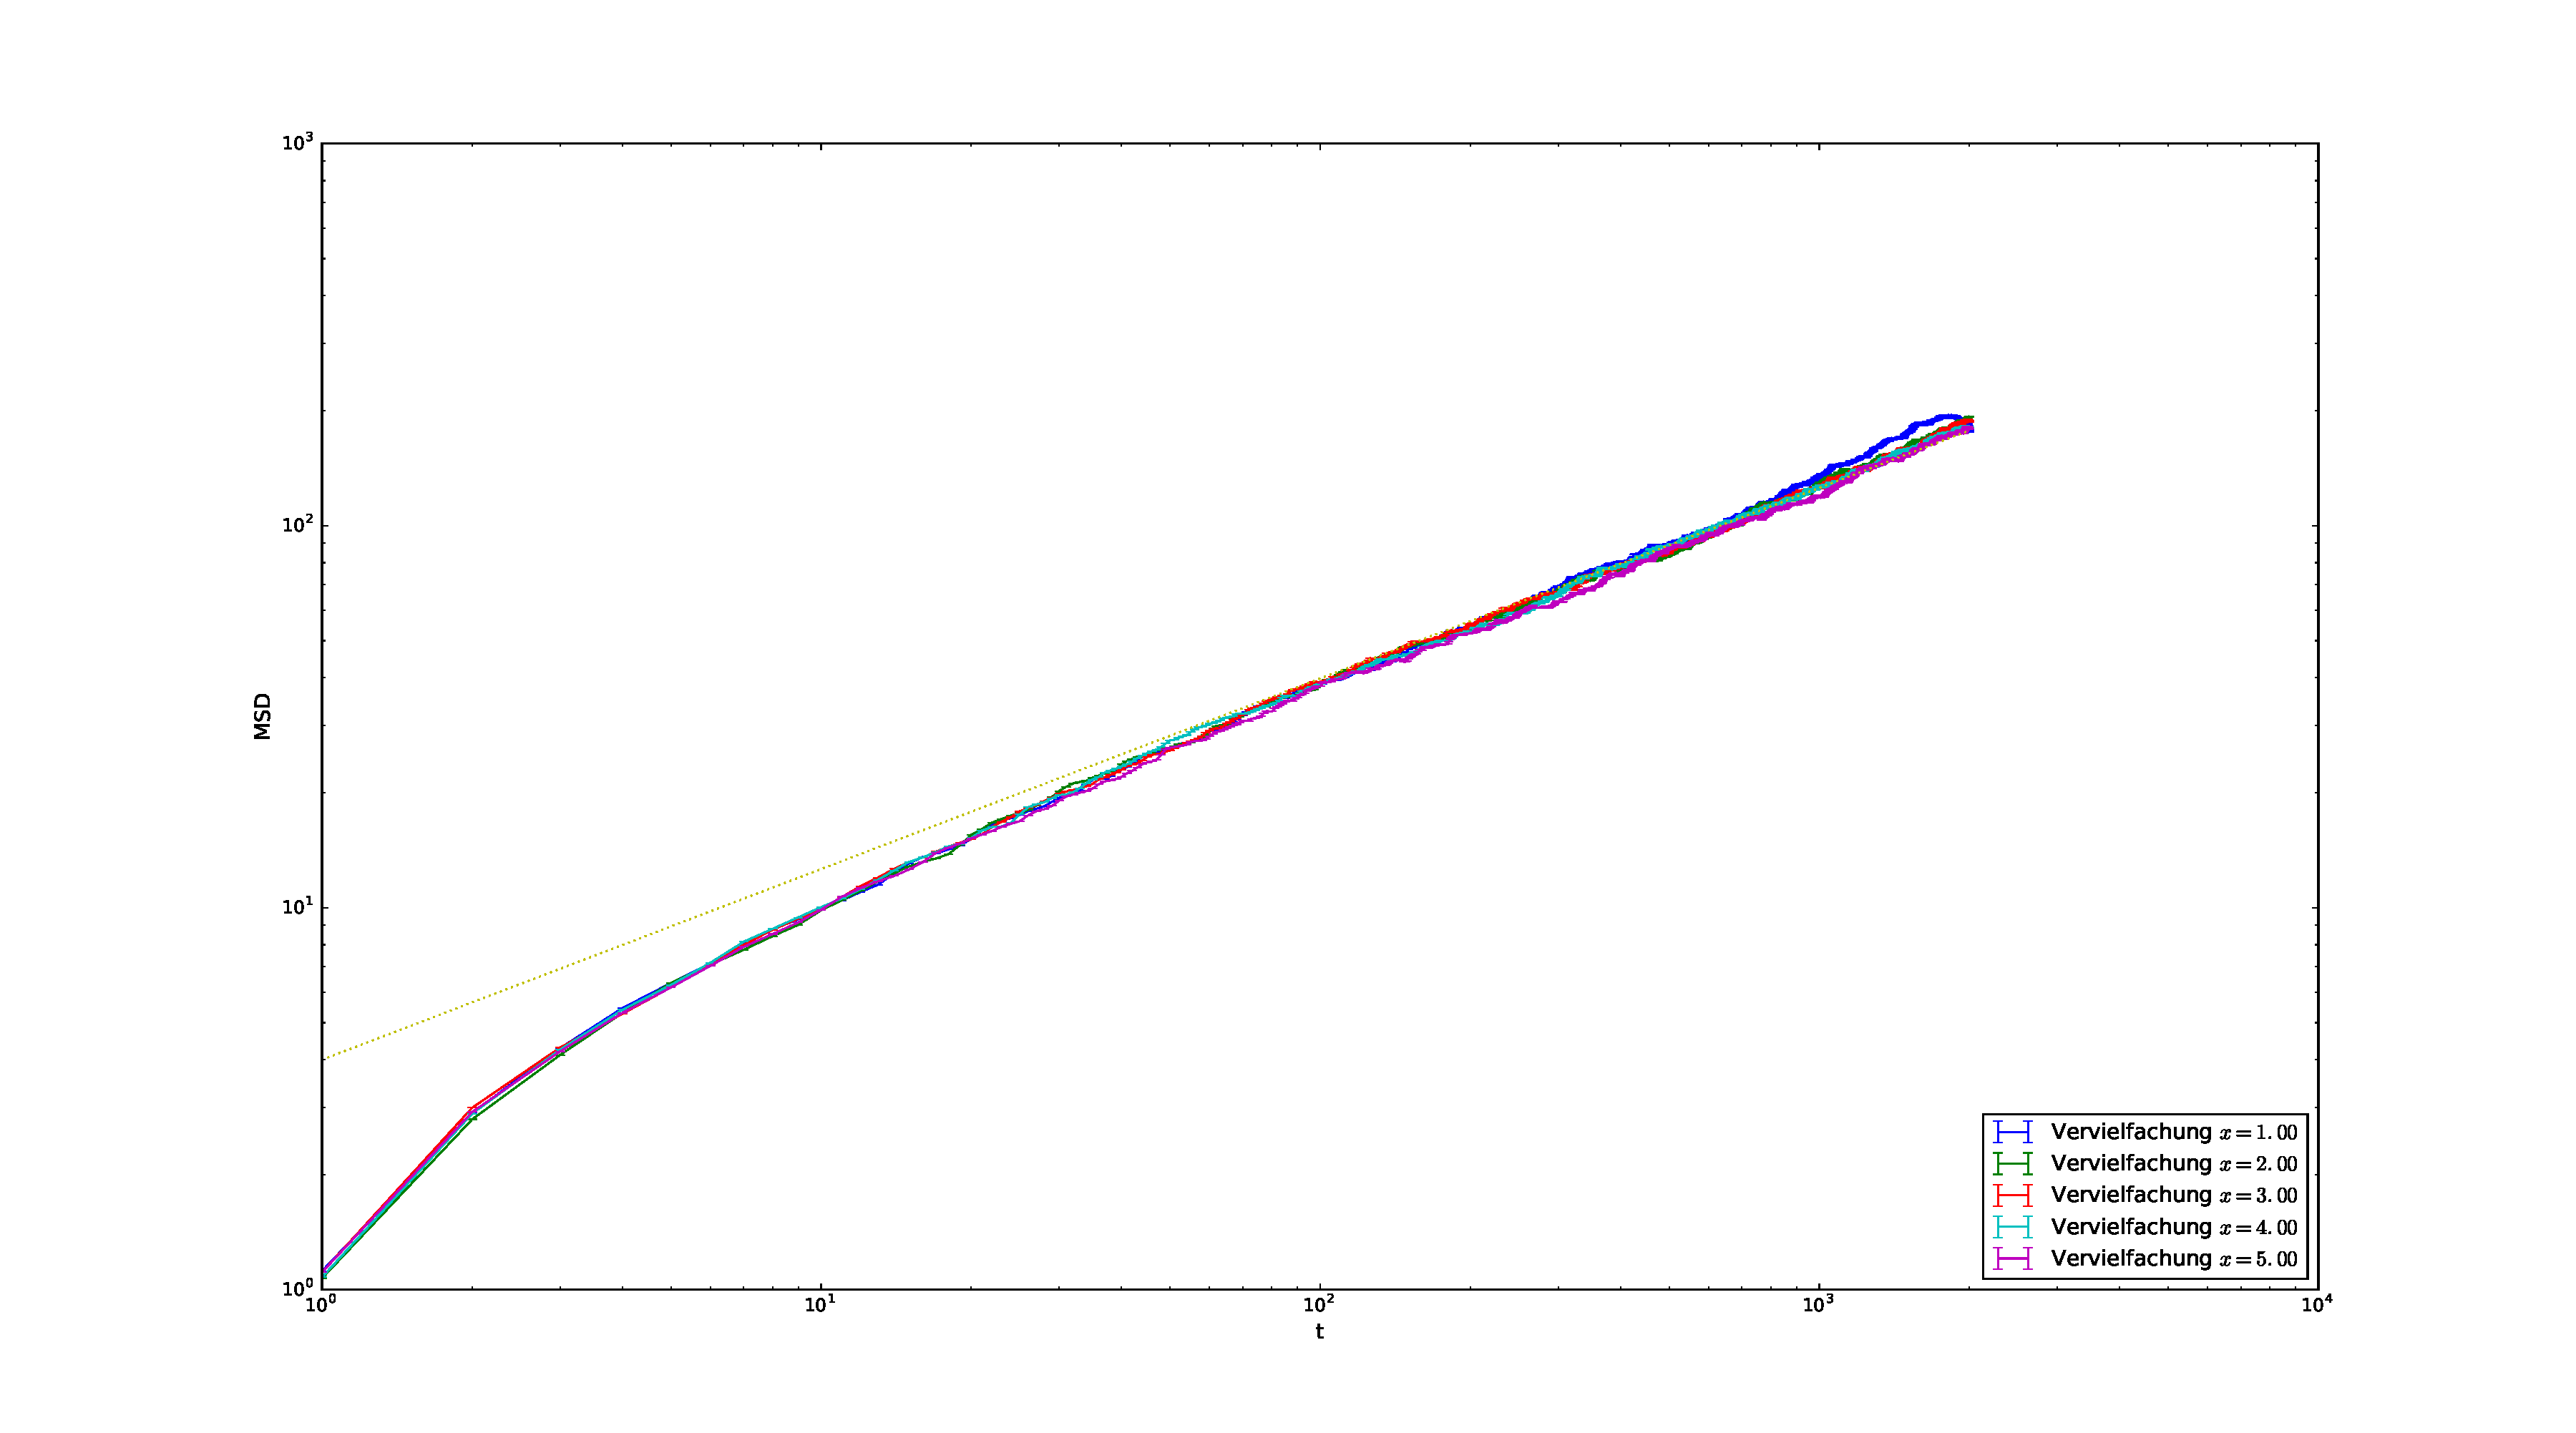
\includegraphics[width=\textwidth]{./faktor_variert_bei_dt_1_log.pdf}
\caption{variere Faktor bei gleichem dt, logarithmisch}
% msd_ensemble_4000particles_log.pdf: 0x0 pixel, -2147483648dpi, 0.00x0.00 cm, bb=
 \centering
\end{figure}

\chapter{Reactions-Diffusion-Dynamics}
\chapter{Status Quo \& Outlook}
\chapter{Appendix}
\subsection{Code:Gebrochen-rationale Brownische Bewegung}
\lstinputlisting[language=Python]{../simulation.py}

\nocite{}

%\printindex
\bibliography{literatur}
\bibliographystyle{plain}
inspired by \url{http://wwo.weizmann.ac.il/weizsites/mukamel/files/2013/01/Brownian_Motion.pdf}

\end{document}